\chapter{Event generation, simulation and reconstruction \label{chap:event_generation}}

\textcolor{red}{Outline to be finalized}

\section{What is an ``event''? \label{sec:event}}

% add picture of CMS event display
% add picture of hadronization etc for event

\section{Event generation \label{sec:event_generation}}

% add info on Madgraph, pythia, jet matching etc

\subsection{Matrix element generators}

\subsection{Parton shower and hadronization}

\subsection{Jet matching}


\section{Event simulation \label{sec:event_simulation}}

\subsection{CMS Full Simulation using Geant4 \label{subsec:fullsim}}

% add some info on how this is done, particle interaction with matter, ionization, 
% how it deals with long lived particles?

\subsection{CMS Fast Simulation \label{subsec:fastsim}}

% explain what approximations are made, why it is necessery, especially in SUSY searches

\section{Event reconstruction \label{sec:event_reconstruction}}

% Add subsection on each object with all the object definitions we use

% We select events with at least one interaction vertex, associated with at least 4 charged-particle
% tracks, that lies within 24~cm of the origin of the CMS coordinate system along the beam direction
% and 2~cm from the origin in the plane transverse to the beam. Owing to the high luminosity of the
% LHC, hard scattering events are typically accompanied by many additional events arising from the
% multiple proton-proton interactions that occur when the proton bunches cross.  The overlapping of
% events is referred to as pileup.  The primary vertex is identified as the vertex with the highest
% value of the $\sum \pt^2$ of the associated tracks.  Detector- and beam-related cleaning algorithms
% are used to remove events with detector noise that mimic events with high energy and large imbalance
% in transverse momentum.  


 

\subsection{Particle Flow technique \label{sec:event_reco_pf}}

% CMS reconstructs events using the particle flow (PF) method~\cite{PF}, which reconstructs particles
% (PF candidates) by combining information from the inner tracker, the calorimeters, and the muon
% system.  Each PF candidate is a ssigned to one of five object categories: muons, electrons, photons,
% charged hadrons, and neutral hadrons.  Contamination from pileup events is reduced by discarding
% charged PF candidates that are incompatible with having originated from the primary
% vertex~\cite{CMS-PAS-JME-14-001}.   The average pileup energy due to neutral hadrons is computed
% event-by-event and subtracted from the energy when computing lepton isolation and jet energy.  The
% energy subtracted is  the average pileup energy per unit area (in $\Delta\eta \times \Delta\phi$)
% times the jet area~\cite{Fastjet1, Fastjet2}.

\subsection{Object identification}

The event selection is an integral part of any physics analysis. It determines which events are
used, and thus what processes contribute to the data sample. This in turn drives how the
backgrounds are estimated, what the sensitivity will be, et cetera. 
An event selection is most easily described in terms of particles, e.g. two electrons, no muons, at
least four jets, as this is the closest to how we think about a given process.  
The particle flow technique is very compatible with this approach, given that it already
reconstructs particles out of the detector hits. 
However, a more thorough selection of the PF objects is needed in order to ensure that their
behaviour is understood, and to ensure that the selected events are not dominated by
misidentified particles, or detector artefacts. 
The physics object groups (POG's) within the CMS Collaboration are in charge of providing general
recommendations on how to define each object. 
In the following paragraphs all the standard objects that will be used in the razor boost analysis
will be discussed.

% 
% Missing transverse energy, which is used in the calculation of the razor variable $\mr$, is 
% defined to be the negative sum of the transverse momenta of all the particle flow objects in an
% event.  Loosely identified and isolated electrons with $\pt > 5$~\GeV and $|\eta| < 2.5$ and muons
% with $\pt > 5$\GeV and $|\eta| < 2.4$ are used both to suppress backgrounds in our signal region and
% in the definition of the control regions.  A tight definition of isolated leptons (electrons with
% $\pt > 10$~\GeV and $|\eta| < 2.5$ and muons with $\pt > 10$~\GeV and $|\eta| < 2.4$) defines a
% control region enriched in $\cPZ \rightarrow \ell \ell $ events, from which we estimate the
% systematic uncertainty in the predicted number of $\cPZ \rightarrow \nu \nu$ events in the signal
% region. Any electron candidates with $1.44 < |\eta| < 1.57$ are rejected since the transition region
% between barrel and endcap calorimeters is less well-instrumented.
% In order to suppress the decays of taus and other leptons that fail the loose selection, events that
% have isolated tracks with $\pt > 10$\GeV and track-primary vertex distance along the beam direction
% $dz < 0.05$ are rejected.


%%%%%%%%%%%%%%%%%%%%%%%%%%%%%%%%%%%%%%%%%%%%%%%%%%%%%%%%%%%%%%%%%%%%%%%%%%%%%%%%%%%%%%%%%%%%%%%%%

%%%%%%%%%%%%%%%%%%%%%%%%%%%%%%%%%%%
%%  Object identification
%%%%%%%%%%%%%%%%%%%%%%%%%%%%%%%%%%%



% The average pileup energy due to neutral hadrons is computed
% event-by-event and subtracted from the energy when computing lepton isolation and jet energy.  The
% energy subtracted is  the average pileup energy per unit area (in $\Delta\eta \times \Delta\phi$)
% times the jet area~\cite{Fastjet1, Fastjet2}.
% this corrects energy and momentum, not substructure
% TODO: move to jet and lepton sections

% 
% Missing transverse energy, which is used in the calculation of the razor variable $\mr$, is 
% defined to be the negative sum of the transverse momenta of all the particle flow objects in an
% event.  Loosely identified and isolated electrons with $\pt > 5$~\GeV and $|\eta| < 2.5$ and muons
% with $\pt > 5$\GeV and $|\eta| < 2.4$ are used both to suppress backgrounds in our signal region
%and
% in the definition of the control regions.  A tight definition of isolated leptons (electrons with
% $\pt > 10$~\GeV and $|\eta| < 2.5$ and muons with $\pt > 10$~\GeV and $|\eta| < 2.4$) defines a
% control region enriched in $\cPZ \rightarrow \ell \ell $ events, from which we estimate the
% systematic uncertainty in the predicted number of $\cPZ \rightarrow \nu \nu$ events in the signal
% region. Any electron candidates with $1.44 < |\eta| < 1.57$ are rejected since the transition
%region
% between barrel and endcap calorimeters is less well-instrumented.
% In order to suppress the decays of taus and other leptons that fail the loose selection, events
%that
% have isolated tracks with $\pt > 10$\GeV and track-primary vertex distance along the beam
%direction
% $dz < 0.05$ are rejected.

\subsubsection{Primary vertices \label{sec:object_vertex}}

We require at least one {\it good} primary vertex to be reconstructed in each event. 
This vertex should be associated with at least four charged-particle tracks. It should also lie
within 24\cm of the origin of the CMS coordinate system along the beam direction, and within 2\cm
in the plane transverse to the beam. 
These requirements, translated to the CMS nomenclature, are summarized in
Table~\ref{tab:object_vertex}.
In case there are multiple good vertices, we choose the vertex with the highest value of $\sum
\pt^2$ of associated tracks to be the leading primary vertex in the event. This vertex is
taken as a reference to reconstruct the event, e.g. to perform the track subtraction for pileup
removal, for which we use the charged hadron subtraction algorithm, as explained before.

\begin{table}[htdp]
\caption{Vertex selection criteria. \label{tab:object_vertex}}
\begin{center}
\begin{tabular}{l l}
\toprule
\texttt{\small isFake()} & $= 0$ \\
\texttt{\small ndof()} & $> 4$ \\
\texttt{\small z()} & $< 24\cm$ \\
\texttt{\small position.Rho()} & $< 2\cm$ \\
\bottomrule
\end{tabular}
\end{center}
\end{table}


\subsubsection{Jets \label{sec:object_jets}}

Most analyses are interested primarily in the quarks and gluon produced in the hard interaction, or
in the decay of heavy particles, such as top quarks or $\W$ bosons. 
However, through the process of parton showering and hadronization, the few initial quarks and
gluons turn into a multitude of hadrons. 
Hadrons from a given initial quark or gluon can usually be found close together, they form a
\textit{jet}. The proper description of jets, and the jet definitions that are used to reconstruct
them, relies on two properties: infrared, and collinear safety~\cite{Salam:2009jx}.
It is important that a jet definition returns the same set of final jets regardless of whether a
parton underwent a collinear or soft splitting. If this is not the case, i.e. the jet definition is
infrared or collinear unsafe, then one finds that divergencies in the theoretical computation of
jet cross sections do not vanish. 

A jet definition comprises two parts: the jet algorithm that defines in which order particles are
grouped together, and the recombination scheme that defines how to combine the momenta of the
to-be-merged particles. 
For the latter, the most common choice is to simply add the four-vectors of the particles, which
then gives rise to massive jets. 
For the jet algorithm there are many choices. Here I will focus solely on the anti-$k_\textrm{T}$
algorithm~\cite{antikt}, which is the default jet algorithm used by CMS.
As for most sequential recombination algorithms, one defines distances $d_{ij}$ between particles
$i$ and $j$ (or pseudojets if particles have been combined before),  and distances $d_{iB}$ between
particle $i$ and the beam.
The distance measures are in this case given by
\begin{align}
  d_{ij} &= \min \left(\frac{1}{p_{\mathrm{T,i}}^2}, \frac{1}{p_{\mathrm{T,j}}^2}\right)
\frac{\Delta R_{ij}^2}{R^2}, \\
  d_{iB} &= \frac{1}{p_{\mathrm{T,i}}^2},
\end{align}
where $\Delta R_{ij}^2 = (y_i - y_j)^2 + (\phi_i - \phi_j)^2$ and $R$ is a tuneable parameter
determining the size of the jets. The rapidity $y$ of a particle is given by,
\begin{equation}
  y = \frac{1}{2} \ln{\frac{ E + p_z }{ E - p_z }} . \label{eq:rapidity}
\end{equation}
The jet clustering proceeds by identifying the smallest of all distances. If it is a $d_{ij}$, we
recombine particles $i$ and $j$, while if it is $d_{iB}$, we move $i$ from the list of particles to
the list of final jets. All distances are then recalculated and the procedure is repeated until no
particles are left.
The anti-$k_\textrm{T}$ algorithm results in mostly circular jets, reminiscent of the older cone jet
algorithms that are no longer used because they are not infrared and collinear safe.

The input to the jet clustering are the PF candidates that pass the charged hadron subtraction. 
The clustering itself is done with the anti-$k_\textrm{T}$ algorithm with size parameter $R=0.5$
(AK5), as implemented in \textsc{FastJet 3.0.1}~\cite{Cacciari:2011ma}.
We apply the standard loose identification criteria to the resulting jets, as defined by the
requirements listed in Table~\ref{tab:object_jets}. Jets are required to not be composed of only a
single component, as this usually indicates that the reconstruction is of poor quality. 

Unfortunately, the calorimeter response to incident particles is not uniform. It is, therefore, not
straightforward to translate the measured jet energy to the true particle energy, which is what we
want to use to do our analysis. A set of jet energy scale corrections -- scalings of the
jet four-momentum depending on jet \pt and $\eta$ -- are applied to both data and
simulation in order to achieve a proper mapping to the particle level. 
Jet energy corrections within CMS are taken care of in a sequential way, each level of correction
taking care of a different effect~\cite{JEC,Chatrchyan:2011ds}. 
The uncertainties associated with the jet energy scale corrections need to be taken into account as
systematic uncertainty on any analysis result. How this will be done in the razor boost analysis is
explained in Section~\ref{sec:boost_JEC}.  

First, the residual effect from pileup is removed using the \textit{L1 corrections}. 
The effect of pileup on a given jet is quantified by the so-called offset, defined as the
difference in \pt for a reconstructed jet with added pileup and the same jet without pileup.
The effects of charged hadrons from in-time pileup have already been largely reduced by the charged
hadron subtraction method. The effect of neutral particles and out-of-time pileup is removed at this
stage using a slightly modified version of the \textit{jet area method}~\cite{Fastjet1,Fastjet2}.
This method uses the effective area of the jets, $A$, multiplied by the average energy density
in the event, $\rho$, to calculate the energy to be subtracted from the jets.
Both real and simulated jets are first corrected with a $\pt$, $\eta$, and number of primary
vertices dependent offset correction determined in simulation. For data events, an additional
data/simulation scale factor is derived from ZeroBias data to correct for remaining $\eta$ dependent
discrepancies.
Figure~\ref{fig:JEC_L1} shows the size of the energy offset for AK5 jets in the central region,
before and after the L1 corrections have been applied. A clear reduction of the overall offset is
observed. The dependence on the number of pileup interaction has also been reduced, indicating that
the L1 corrections behave properly.  

\begin{figure}[tpb]
  \centering
  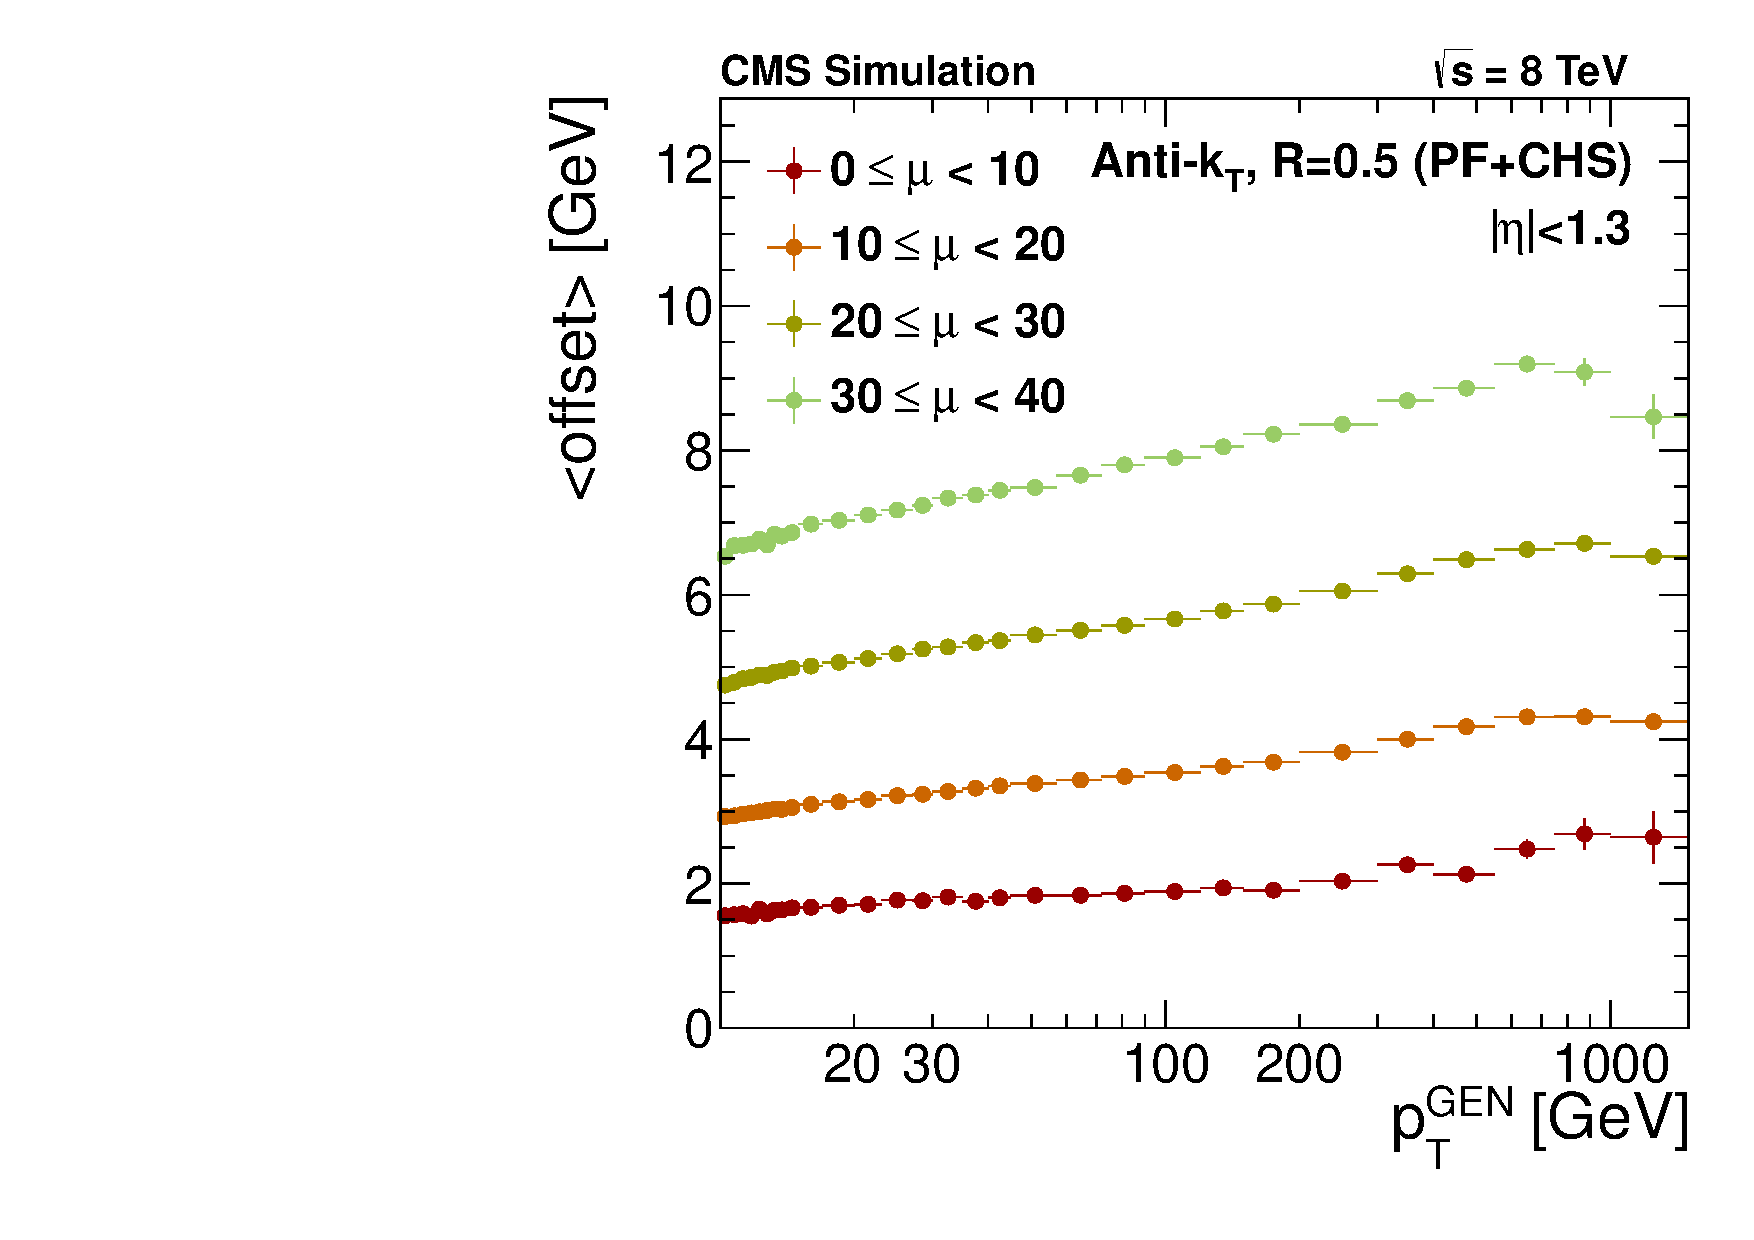
\includegraphics[width=0.4\textwidth]{figures/eventreco_objects/OffMeantnpuRef_BB_ak5pfchs}
  ~
  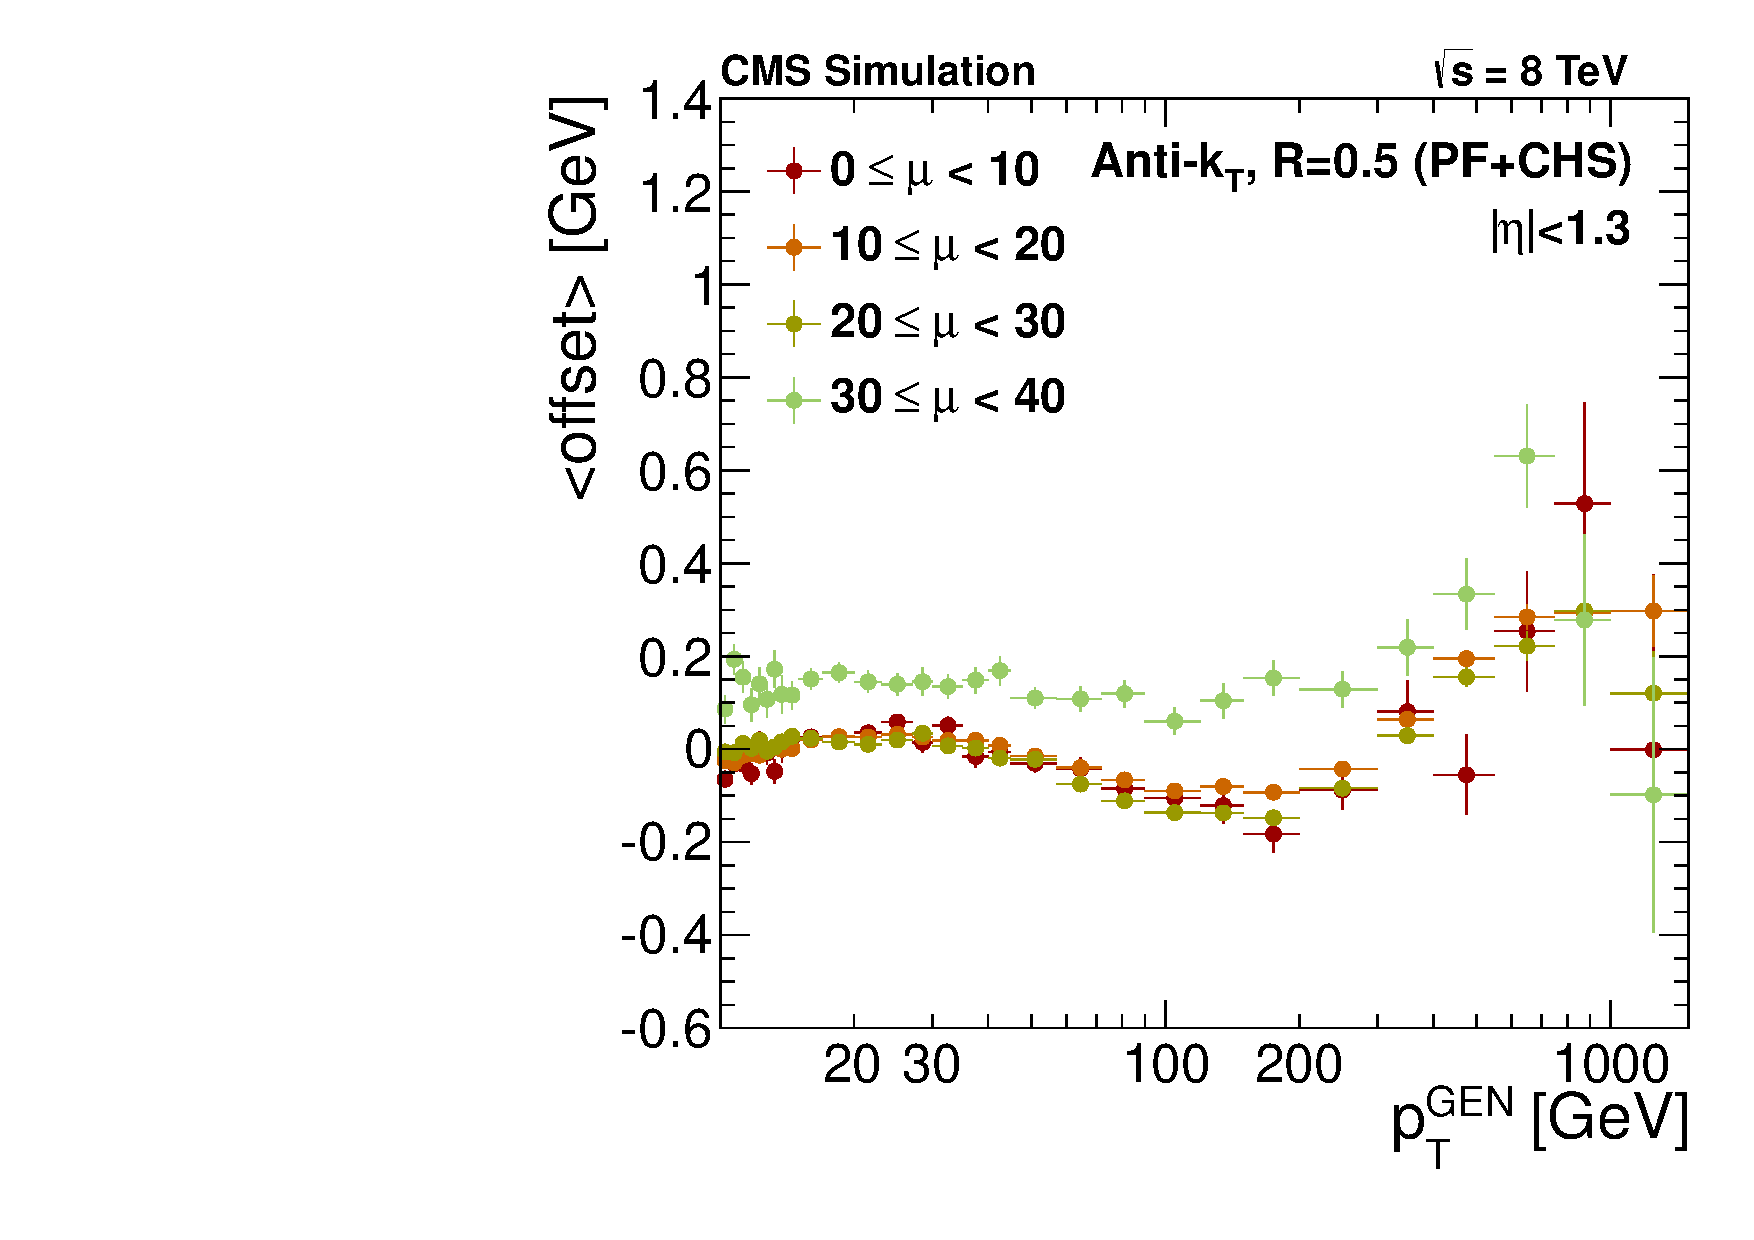
\includegraphics[width=0.4\textwidth]{figures/eventreco_objects/OffMeantnpuRef_BB_ak5pfchsl1}
  \caption{The offset shown on the $y$-axis in these plots is defined as the difference in
transverse momentum for a reconstructed jet with added pileup and the same jet without pileup.
The left-hand side shows the offset as a function of the generated \pt of a jet before the L1
corrections have been applied, and the right-hand side shows the offset after pileup
corrections. Different markers represent different levels of pileup. Figures taken from
Ref.~\cite{JEC_plots}.
  \label{fig:JEC_L1}}
\end{figure}

Since the simulation of the detector response is very detailed, see
Section~\ref{sec:event_simulation}, the jet response in the absence of pileup is in fact very well
modelled in simulation. The bulk of the jet energy corrections will thus be derived using
simulation, and only the residual differences between data and simulation are derived directly
from the data.

The second and third level of corrections, the \textit{L2 Relative} and \textit{L3 Absolute
corrections}, are designed to make the jet response flat in $\eta$ and \pt, respectively. They are
derived from the simulation together. The L2 correction corrects a jet at arbitrary $\eta$ relative
to a jet in the central area ($|\eta|<1.3$). Once that is done, the jet energy is translated back to
the particle level, such that on average the \pt of a reconstructed jet matches that of a jet
clustered using generator level particles,
\begin{equation}
  <\pt(\mathrm{reco})_{\mathrm{corr}}> {=} <\pt(\mathrm{gen})> .
\end{equation}
These are the final corrections applied to jets from simulated events. The size of the L2 and L3
corrections as a function of jet $\eta$, for three reference \pt values, is shown in
Fig.~\ref{fig:JEC_L23} on the left-hand side. 

\begin{figure}[tpb]
  \centering
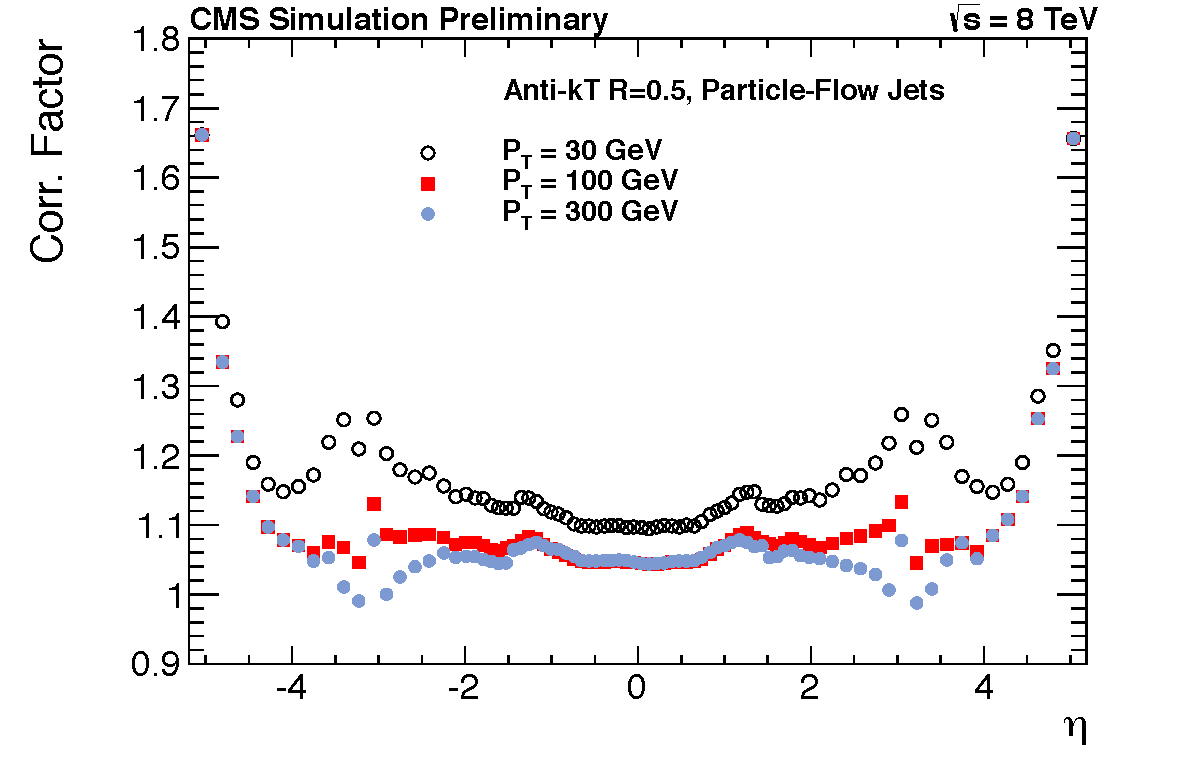
\includegraphics[height=0.22\textheight]
{figures/eventreco_objects/CorrectionVsEta_Overview_TDR_ak5pfl1_L2L3}
~
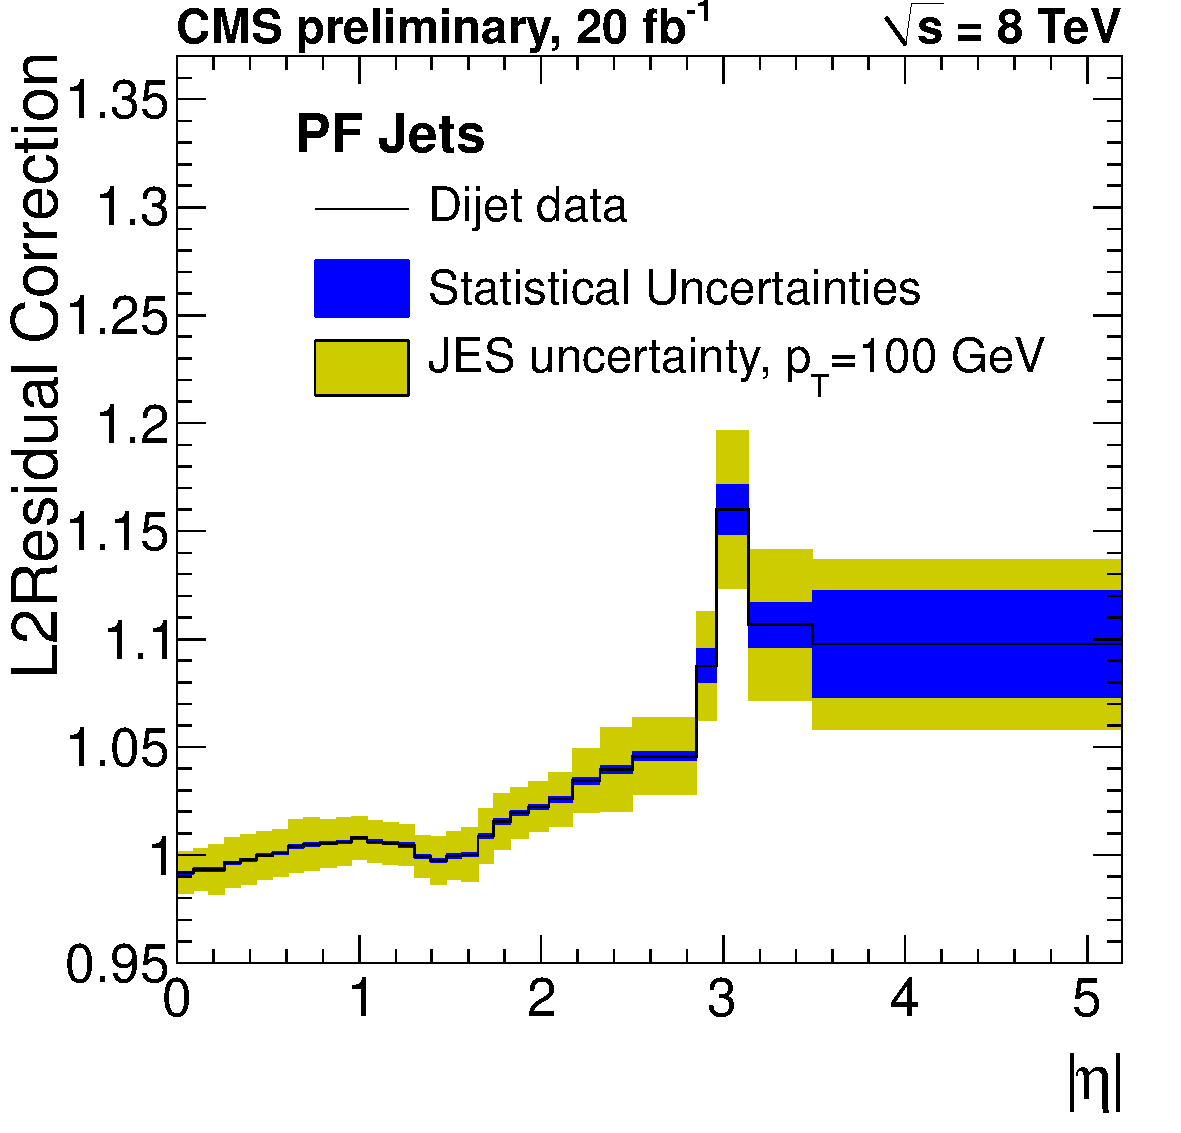
\includegraphics[height=0.22\textheight]
  {figures/eventreco_objects/ResComp_FSRcorr_residuals_Abseta_PF_DiJetData}
  \caption{[left] The size of the L2 and L3 corrections as a function of jet $\eta$ for three
reference transverse momentum values: 30\GeV (white hollow circles), 100\GeV (red squares) and
300\GeV (blue circles). 
[right] L2 Residual corrections, obtained from dijet events, as a function of $\eta$. The jet
energy scale uncertainty is shown with a yellow band, while the statistical uncertainty is shown
with a blue band.
Figures taken from Ref.~\cite{JEC_plots2}.
  \label{fig:JEC_L23}}
\end{figure}

Data events are further corrected by the \textit{L2L3 Residual} jet energy scale
\textit{corrections} to take care of the small differences between data and simulation. These
corrections are \pt and $\eta$ dependent, and only correct the relative energy scale. The absolute
energy scale was found to be well modelled in the simulation. A dedicated, data-driven approach is
employed, using data samples of dijet, $\gamma+$jet, and $\cPZ+$jet events. The L2 Residual
correction derived from dijet events is shown on the right in Fig.~\ref{fig:JEC_L23}.

After all corrections have been applied, jets to be used for analysis are required to have $\pt >
30\GeV$ and $|\eta| < 2.4$.
The AK5 jets defined in this section will be used for most aspects of
the razor boost analysis, except for the reconstruction of boosted hadronic $\W$-candidates. 
Section~\ref{sec:boost_wtag} provides details on the dedicated jet treatment that is used for $\W$
tagging.

\begin{table}[htdp]
\caption{Jet selection criteria. \label{tab:object_jets}}
\begin{center}
\begin{tabular}{l l}
\toprule
\pt & $> 30\GeV$ \\
$|\eta|$ & $< 2.4$ \\
\midrule
\texttt{\small neutralHadronEnergyFraction()} & $< 0.99$ \\
\texttt{\small neutralEmEnergyFraction()} & $< 0.99$ \\
\texttt{\small nConstituents()} & $> 1$ \\
\texttt{\small chargedHadronEnergyFraction()} & $> 0$ \\
\texttt{\small chargedMultiplicity()} & $> 0$ \\
\texttt{\small chargedEmEnergyFraction()} & $< 0.99$ \\
\bottomrule
\end{tabular}
\end{center}
\end{table}

%%%%%%%%%%%%%%%%%%%%%%%%%%%%%%%%%%%%%%%%%%%%%%%%%%%%%%%%%%%%%%%%%%%%%%%%%%%%%%%%%%%%%%%%%

\subsubsection{B-tagging \label{sec:object_btag}}

Jets originating from the hadronization of $\cPqb$ quarks can be distinguished from other jets,
initiated by gluons or light flavour quarks, due to the long lifetime, of the order of
1.5\ten{-12}\second, of the $B$ hadrons. 
The non-prompt decay of the $B$ hadrons results in a secondary vertex, displaced by hundreds of
micrometers with respect to the primary vertex of the hard interaction. This feature can be used to
identify jets as originating from a $\cPqb$ quark. 

The ability to distinguish $\cPqb$ jets is especially important for new physics searches. Many new
physics models are associated with production of third generation quarks, whereas this is more rare
in the standard model. For many searches $\cPqb$ jet tagging is an essential tool in suppressing
the background from multijet or vector boson production. 

CMS has developed several $\cPqb$ tagging algorithms\cite{btag7TeV,btag8TeV}. The combined
secondary vertex (CSV) algorithm is the most widely used, and combines information on the secondary
vertices and the impact parameter of the tracks into a likelihood based discriminant. 
 
The input to any $\cPqb$ tag algorithm are high purity tracks, which feature a good track fit with
many separate hits, have $\pt > 1\GeV$, and lie within the jet cone. 
The impact parameter of a track is defined as the distance from the primary vertex to the track at
the point of closest approach.  
Secondary vertices within jets are reconstructed using an adaptive vertex
fitter~\cite{Fruhwirth:2007hz}. The list of secondary vertices is cleaned from candidates that
share more than 65\% of their tracks with the primary vertex of the event. Vertices that are
consistent with originating from a $K^0$ decay are also removed. Properties of the secondary
vertices used in the CSV likelihood discriminant are the flight distance between secondary and
primary vertex, the flight distance significance, the vertex invariant mass, and the total \pt of
all associated tracks. The impact parameter of the tracks is also included. The shape of the CSV
discriminant, and a data versus simulation comparison, is shown on Fig.~\ref{fig:CSV_discriminant}.

In the razor boost analysis the CSV $\cPqb$ tagging algorithm will be applied on the PF jets at two
working points~\cite{BTagWP}, which are shown on Table~\ref{tab:object_btag}. 
The Loose working point (CSVL), corresponding to a misidentification rate of $\sim$10\% and
efficiency of $\sim$85\%, will be used to veto $\cPqb$ jets, whereas the Medium working point
(CSVM), corresponding to a misidentification rate of $\sim$1\% and a typical efficiency of
$\sim$70\% , is used to select $\cPqb$ jets.
The small differences in the discriminant shape, as observed from Fig.~\ref{fig:CSV_discriminant}, 
will result in a slightly different $\cPqb$ tagging efficiency in data versus simulation. Scale
factors (SF) with associated uncertainties have been derived to correct for this effect, and are
provided by the BTAG POG in CMS. Section~\ref{sec:boost_btag_sf} will cover how these
uncertainties are propagated to the final systematic uncertainties for the razor boost analysis. 

\begin{figure}[tpb]
  \centering
  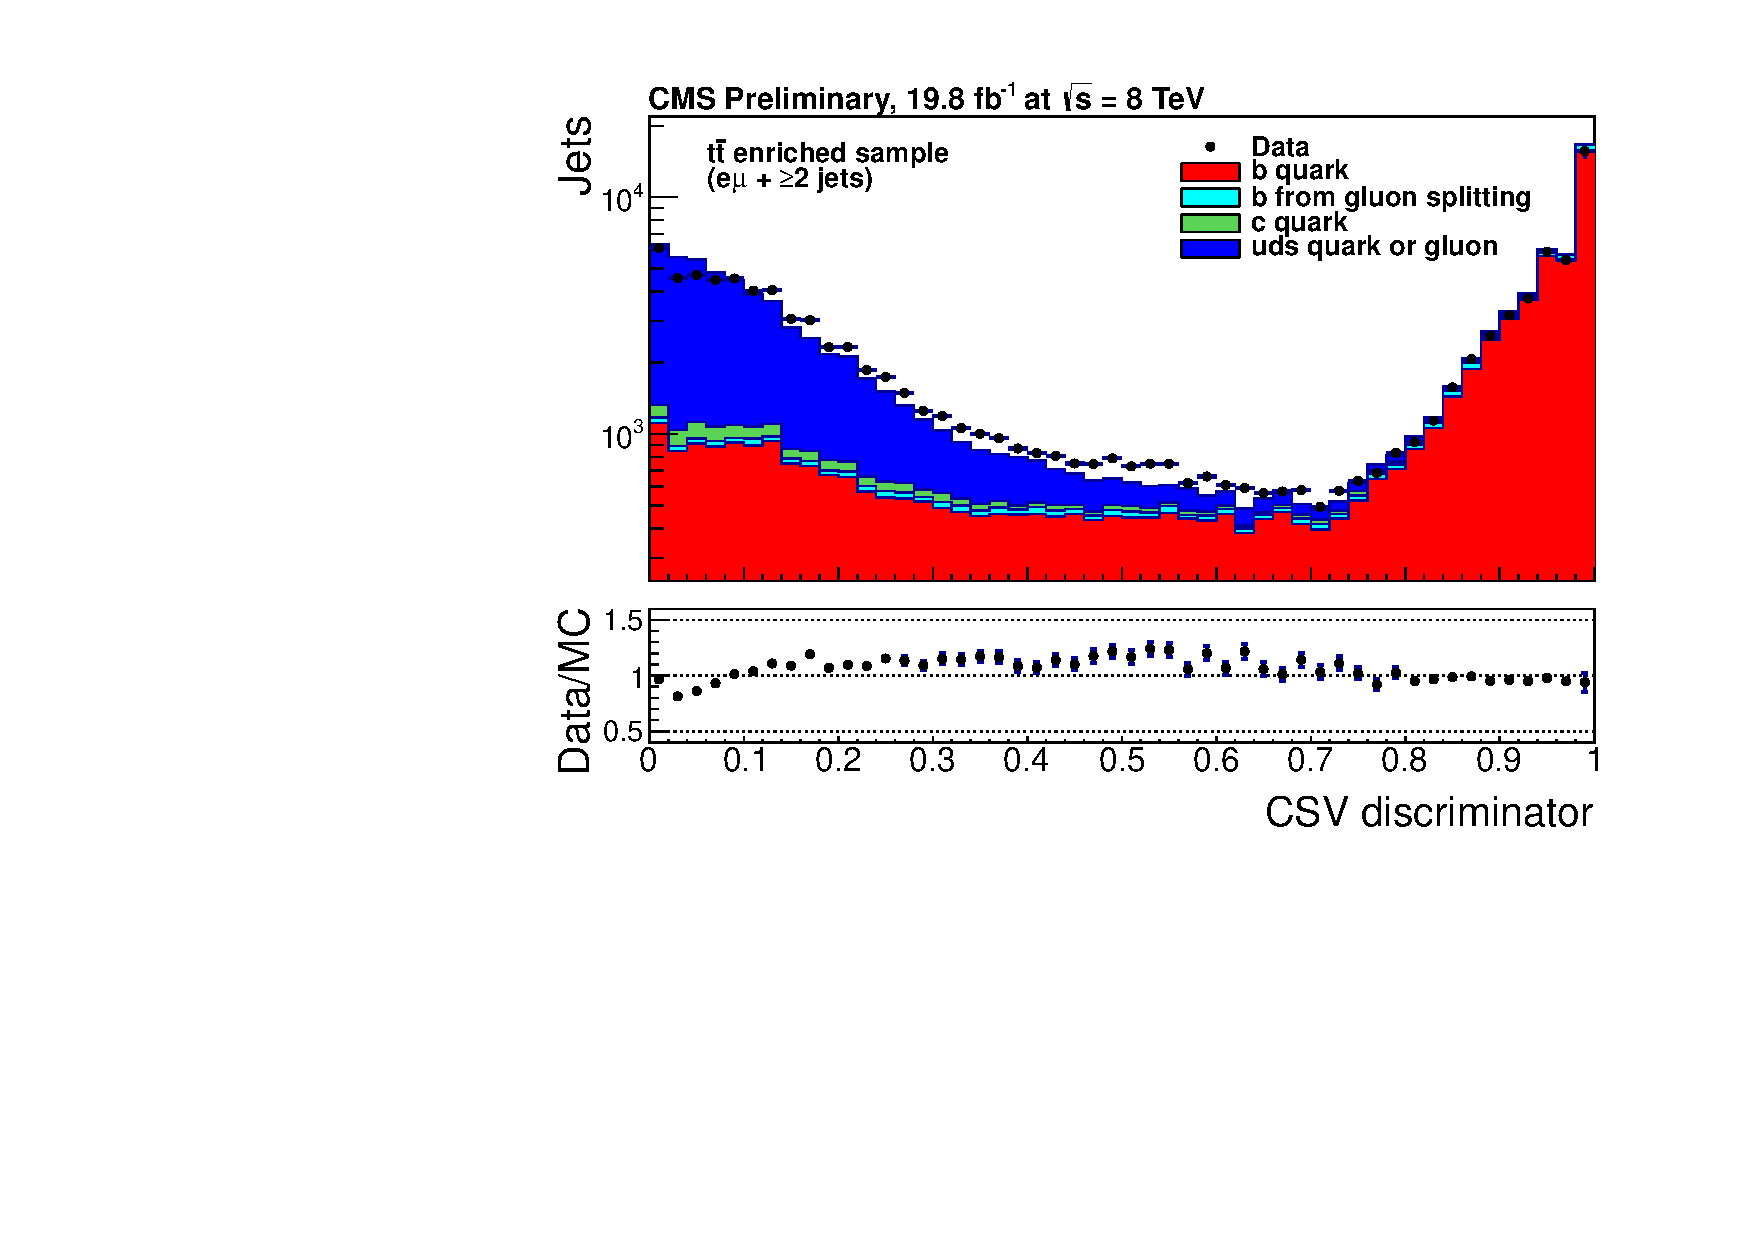
\includegraphics[width=0.6\textwidth]{figures/eventreco_objects/CSV_Log_ttbar}
  \caption{ Discriminator value for the CSV discriminant for a $t\bar{t}$-enriched data sample.
  \label{fig:CSV_discriminant}}
\end{figure}

\begin{table}[htdp]
\caption{Working points for the combined secondary vertex $\cPqb$ jet tagger.
\label{tab:object_btag}}
\begin{center}
\begin{tabular}{l l}
\toprule
Working point & Discriminator value \\
\midrule
Medium & $> 0.679$ \\
Loose & $> 0.244$ \\
\bottomrule
\end{tabular}
\end{center}
\end{table}


%%%%%%%%%%%%%%%%%%%%%%%%%%%%%%%%%%%%%%%%%%%%%%%%%%%%%%%%%%%%%%%%%%%%%%%%%%%%%%%%%%%%%%%%%

\subsubsection{Muons \label{sec:object_muon}}

The razor boost analysis uses muons that are identified using two different working
points, a loose selection and a tight selection, both of which will be detailed below. 
The loose selection is used throughout most of the analysis, both for vetoing the presence of muons
in the signal region, and for selecting single muon events in the control regions. The tight
selection is used only to define a control region enriched in $\cPZ\rightarrow
\ell\bar{\ell}$ events which is used to derive a systematic uncertainty on the contribution of
$\cPZ\rightarrow \nu\bar{\nu}$ in the signal region. 

The \textbf{loose muon selection} was developed especially for events with a
large amount of hadronic activity, where the standard identification criteria were observed to lose
efficiency, resulting in less background suppression when vetoing the presence of muons. 
The details and performance of this optimized selection is documented in
Ref.~\cite{CMS-AN2011-498}. 
The main feature is the use of a so-called \textit{directional isolation}.
The isolation of a particle is a measure of how far it is from other activity in the detector. The
leptons we are interested in, those originating in the hard interaction, are usually separated from
other activity, e.g. jets. This is not the case for misidentified muons or for muons from the decay
of heavy-flavour jets. Directional isolation is designed to have a better rejection of leptons from
these heavy-flavour jet decays, and is defined as
\begin{equation}
\overrightarrow{\mathrm{ISO}}(R) \equiv \sum_{\Delta R_{i} < R} \delta_{i}^{2}\pt{}_{i} ,
\end{equation}
where the sum is over all other particles $i$ within $\Delta R_{i}<R$ of the muon direction,
and $\delta_{i}$ is the angle between particle $i$ and the $\pt$-weighted centroid position
($\delta_{c}$) of all such particles in $(\eta,\phi)$ space. That is, if $\Delta\phi_i$ and
$\Delta\eta_i$ are respectively the difference in $\phi$ and $\eta$ angles between particle $i$ and
the muon, then:
\begin{eqnarray*}
\vec{e}_{i} & \equiv & \frac{1}{\sqrt{\Delta\phi_{i}^{2}+\Delta\eta_{i}^{2}}}\left(\begin{array}{c}
\Delta\phi_{i},\\
\Delta\eta_{i}
\end{array}\right),\\
\vec{\delta}_{c} & = & \sum_{\Delta R_{i}<R}\pt{}_{i}\vec{e}_{i},\\
\delta_{i} & = &
\angle(\vec{\delta}_{c},\vec{e}_{i})=\arccos(\vec{\delta}_{c}\cdot\vec{e}_{i}/|\vec{\delta}_{c}|),
\end{eqnarray*}
where $\vec{e}_{i}$ is the unit vector specifying particle $i$'s relative location in $(\eta,\phi)$
space with respect to the considered muon, as illustrated in Fig.~\ref{fig:object_directional_iso}.
Because of the weighting by $\delta_{i}^{2}$, the value for the directional isolation tends to be
larger for muons that are near the jet core, e.g. in case of leptonic $\cPqb$ decays, compared to
the more conventional isolation definition which does not use this weighting. 

\begin{figure}[htpb]
  \centering
  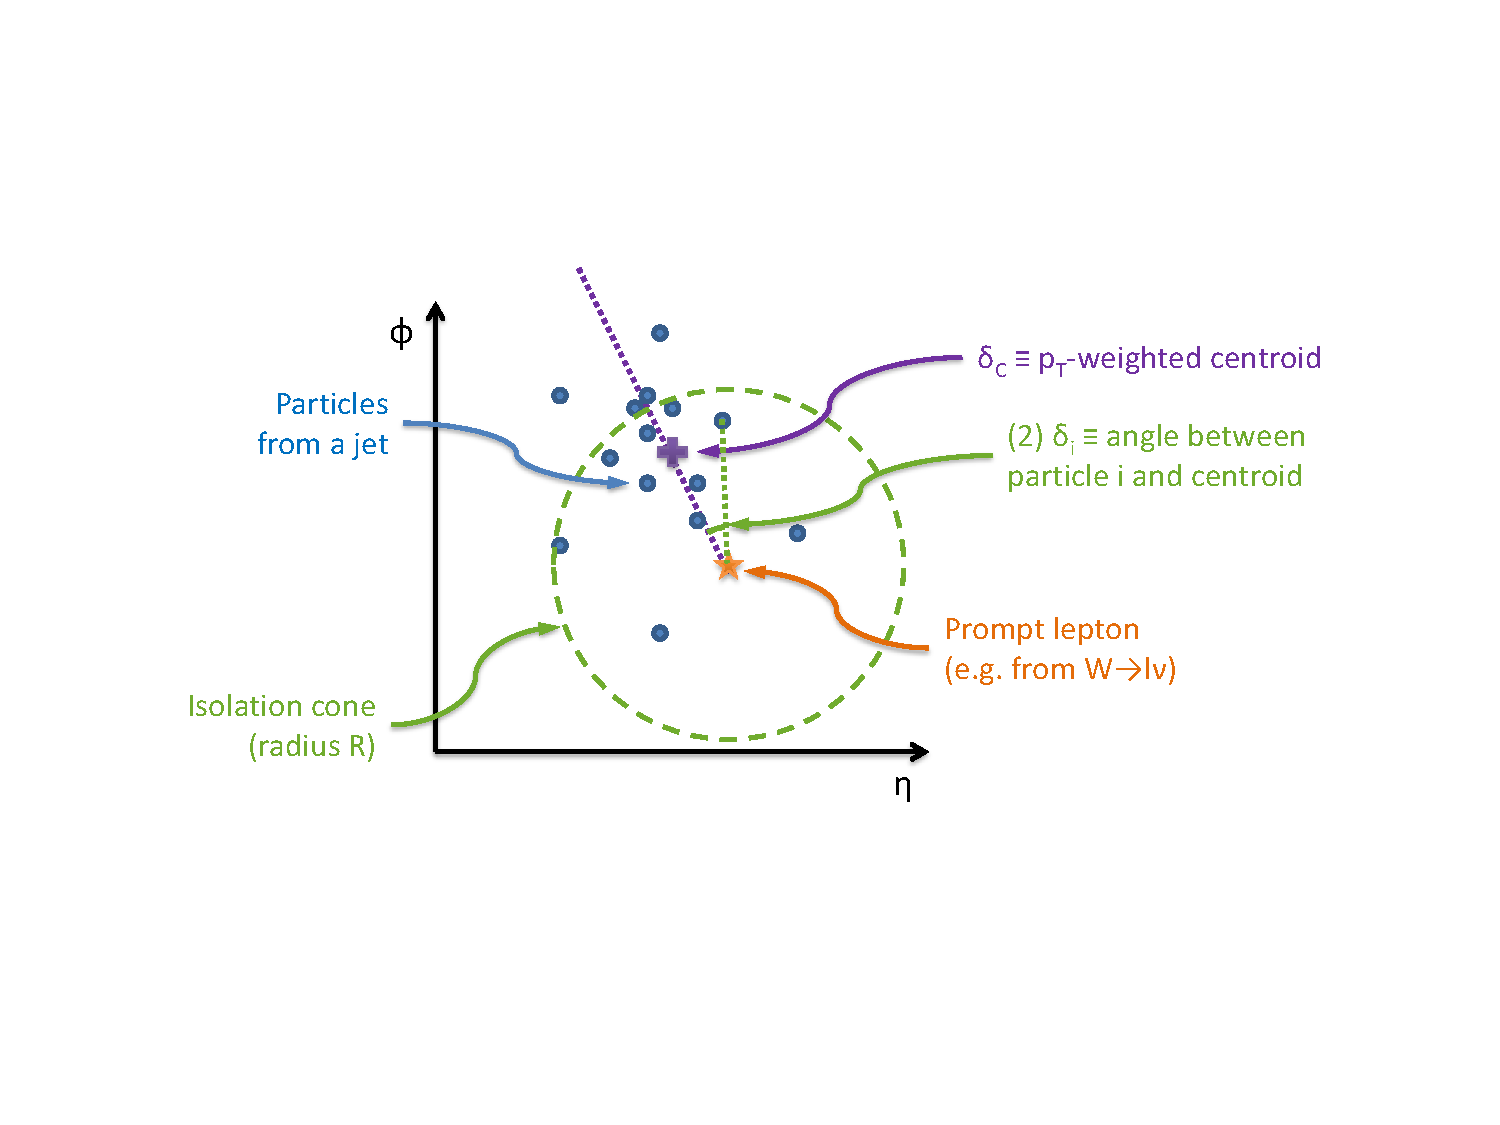
\includegraphics[width=0.8\textwidth]{figures/eventreco_objects/directional_iso_cartoon}
  \caption{Illustration of ingredients used in the computation of directional isolation for a prompt
muon, denoted by a star, near some particles from a jet, denoted by points, in the $(\eta,\phi)$
plane. For prompt leptons $\delta_i$ tends to be small, especially for the high-\pt particles near
the core of the jet. Figure taken from Ref.~\cite{CMS-AN2011-498}.
  \label{fig:object_directional_iso}}
\end{figure}

Apart from the isolation, the identification criteria themselves are also altered from the standard
Loose Muon ID from the POG in order to further optimize the muon identification in environments
with large hadronic activity. 
Loose muons are reconstructed using either the global muon algorithm or the tracker-only
algorithm. 
Global muons are required to pass the {\tt GlobalMuonPromptTight} quality criteria,
and to have at least two muon chambers containing segments uniquely matched to its inner track. 
Tracker-only muons are required to pass the {\tt TMLastStationTight} criteria, which require the
muon to have compatible hits in the last muon chamber. 
All selected muons are then required to pass the selection listed in
Table~\ref{tab:object_loosemuon}. 
Some aspects of the selection depend on the muon $\pt$ and $\eta$; these are summarized in
Table~\ref{tab:object_loosemuon_cuts}.

\begin{table}[p]
\caption{Loose muon definition. }
\begin{center}
{\small
\begin{tabular}{l l}
\toprule
\pt & $> 5\GeV$ \\
$|\eta|$ & $< 2.4$ \\
\midrule
\texttt{\footnotesize innerTrack().hitPattern().numberOfLostHits()} & $\leq 1$ if $\pt < 20\GeV$ \\
                                                      & $\leq 4$ if $\pt \geq 20\GeV$ \\
$|\texttt{\footnotesize innerTrack().dxy(vertex.position())}|$ & $\pt$- and $\eta$-dependent\\
$|\texttt{\footnotesize muonBestTrack().dz(vertex.position())}|$ & $\pt$- and $\eta$-dependent\\
\midrule
$\overrightarrow{\mathrm{ISO}}(R=0.2)$ & $\pt$- and $\eta$-dependent \\
\bottomrule
\end{tabular}
}
\end{center}
\label{tab:object_loosemuon}
\end{table}

\begin{table}[p]
\caption{Details of the $\pt$ dependent thresholds employed in the loose muon selection.}
\begin{center}
  \begin{tabular}{l cccccc }
      \toprule
      Muon $\pt$  & $d_{xy} (\cm)$ & $d_{xy} (\cm)$ & $d_z (\cm)$ & $d_z (\cm)$ &
$\overrightarrow{\mathrm{ISO}}(0.2)$ &
$\overrightarrow{\mathrm{ISO}}(0.2)$ \\
      (\GeV) & Barrel & Endcap & Barrel & Endcap & Barrel & Endcap \\
      \midrule
      0 - 5          & 0.052 & 0.037 & 0.054 & 0.076 & 1.5  & 2    \\
      5 - 10         & 0.041 & 0.018 & 0.042 & 0.082 & 3    & 2.5  \\
      10 - 25        & 0.029 & 0.013 & 0.028 & 0.098 & 7    & 7.5  \\
      15 - 20        & 0.014 & 0.015 & 0.034 & 0.1   & 10.5 & 9    \\
      20 - 40        & 0.021 & 0.021 & 1     & 0.1   & 15.5 & 13.5 \\
      40 - 80        & 0.04  & 0.2   & 1     & 1     & 32.5 & 19   \\
      80 - 140       & 0.1   & 0.2   & 1     & 1     & 54.5 & 37   \\
      140 - 200      & 0.1   & 0.2   & 1     & 1     & 87   & 65.5 \\
      \bottomrule
    \end{tabular}
\end{center}
\label{tab:object_loosemuon_cuts}
\end{table}

 
The \textbf{tight muon selection} follows the recommendation from the Muon POG~\cite{MuonID}.
In addition to the identification criteria, we also require the tight muon to be isolated. 
Here we do not use directional isolation, but rather the more standard particle-based relative
isolation. 
This isolation, denoted $I_\mu$, is calculated using the PF candidates in a cone of size $\Delta R =
0.4$ around the muon. Charged-hadron candidates associated with pileup vertices are not taken into
account in the calculation of the isolation. However, they are used to estimate the remaining
contribution to the isolation coming from neutral hadrons associated with pileup. This contribution
is then subtracted. 
The isolation definition is given by:
\begin{equation}
I_\mu = \frac{I_{Charged} + \max\left(0, I_{Neutral} + I_{\gamma} - \Delta\beta\cdot
I_{Charged}^{PU}\right)}
             {\pt^\mu} , 
\label{eqn:iso}
\end{equation}
where $I_{Charged}$, $I_{Neutral}$, and $I_{\gamma}$ are computed as the sum of the \pt of the
charged hadrons, neutral hadrons and photons, respectively, in a cone of size $\Delta R = 0.4$
around the muon. The parameter $\Delta\beta$ is set to 0.5, and $I_{Charged}^{PU}$ is the estimated
contribution from pileup computed as the sum of the \pt of the charged hadrons associated with
pileup vertices.
The tight muon isolation requirement is $I_\mu < 0.15$.
A summary of the tight muon selection can be found in Table~\ref{tab:object_tightmuon}. 

\begin{table}[p]
\caption{Tight muon definition. }
\begin{center}
{\small
\begin{tabular}{l l}
\toprule
\pt & $> 10\GeV$ \\
$|\eta|$ & $< 2.4$ \\
\midrule
\texttt{\footnotesize isPFMuon()} & $= 1$ \\
\texttt{\footnotesize isGlobalMuon()} & $= 1$ \\
\texttt{\footnotesize globalTrack().normalizedChi2()} & $< 10$ \\
\texttt{\footnotesize globalTrack().hitPattern().numberOfValidMuonHits()} & $> 0$ \\
\texttt{\footnotesize track().hitPattern().trackerLayersWithMeasurement()} & $> 5$ \\
\texttt{\footnotesize innerTrack().hitPattern().numberOfValidPixelHits()} & $> 0$ \\
\texttt{\footnotesize numberOfMatchedStations()} & $> 1$ \\
$|\texttt{\footnotesize innerTrack().dxy(vertex.position())}|$ & $< 0.2\cm$ \\
$|\texttt{\footnotesize muonBestTrack().dz(vertex.position())}|$ & $< 0.5\cm$ \\
\midrule
$I_\mu =$ [\texttt{\footnotesize pfIsolationR04().sumChargedHadronPt()}& \\
\hspace{0.9cm} $+$ max(0., \texttt{\footnotesize pfIsolationR04().sumNeutralHadronPt()}  & \\
\hspace{2.7cm} $+$ \texttt{\footnotesize pfIsolationR04().sumPhotonPt()}  & \\
\hspace{2.7cm} $-$ 0.5 $\cdot$ \texttt{\footnotesize pfIsolationR04().sumPUPt()}) & \\
\hspace{0.9cm} ] / \pt & $< 0.15$ \\ 
\bottomrule
\end{tabular}
}
\end{center}
\label{tab:object_tightmuon}
\end{table}

 
%%%%%%%%%%%%%%%%%%%%%%%%%%%%%%%%%%%%%%%%%%%%%%%%%%%%%%%%%%%%%%%%%%%%%%%%%%%%%%%%%%%%%%%%%


\subsubsection{Electrons \label{sec:object_electron}}

Similar to the muon selection, we identify electrons using two different working points, a loose
selection, and a tight selection. 

The \textbf{loose electron selection} uses directional isolation as described in the previous
section, and fully documented in Ref.~\cite{CMS-AN2011-498}. A summary of the complete
loose electron selection is given in Table~\ref{tab:object_looseelectron}, with the details of
the $\pt$- and $\eta$-dependent requirements listed in Table~\ref{tab:object_looseelectron_cuts}. 

\begin{table}[p]
  \caption{Loose electron definition.}
  \begin{center}
  {\small 
    \begin{tabular}{l l l l}
      \toprule
      & Condition & Barrel & Endcap \\
      \midrule
      \pt & & $ > 5 \GeV$ & $> 5\GeV$ \\
      $|\eta|$ & & $ < 1.442$ & $1.556 - 2.5$ \\
      \midrule
      \texttt{\footnotesize gsfTrack().numberOfLostHits()} & $\pt < 20\GeV$ & $= 0$ & $= 0$ \\
      \texttt{\footnotesize gsfTrack().hitPattern().numberOfValidPixelHits()} & $\pt < 10\GeV$ &
$\geq 2$ & $\geq 1$ \\
      $|\texttt{\footnotesize gsfTrack().dz(vertex.position())}|$ & & \multicolumn{2}{l}{$\pt$- and
$\eta$-dependent}\\
      \midrule
      $\overrightarrow{\mathrm{ISO}}(R=0.3)$, calculated from charged particles only & &
\multicolumn{2}{l}{$\pt$- and $\eta$-dependent} \\
      $\overrightarrow{\mathrm{ISO}}(R=0.2)$, barrel only, calculated using all particles & &
\multicolumn{2}{l}{$\pt$- and $\eta$-dependent} \\
      \bottomrule
    \end{tabular}
    }
  \end{center}
  \label{tab:object_looseelectron} 
\end{table}


\begin{table}[p]
  \caption{Details of the $\pt$ dependent thresholds employed in the loose electron selection.}
  \begin{center}
  \begin{tabular}{ l ccccc }
      \toprule
      Electron $\pt$ & $d_z (\cm)$ & $d_z (\cm)$ &
$\overrightarrow{\mathrm{ISO}}(0.3,\textrm{charged})$ &
$\overrightarrow{\mathrm{ISO}}(0.3,\textrm{charged})$ & $\overrightarrow{\mathrm{ISO}}(0.2)$ \\
      (\GeV) & Barrel & Endcap & Barrel & Endcap & Barrel \\
      \midrule
      0 - 5          & 0.03 & 0.09 & 0.5  & 0.5  & 2    \\
      5 - 10         & 0.05 & 0.09 & 1.5  & 2.5  & 4.25 \\
      10 - 25        & 0.05 & 0.09 & 4.5  & 6.5  & 8.75 \\
      15 - 20        & 0.05 & 0.11 & 7.5  & 9    & 11   \\
      20 - 40        & 0.2  & 1    & 10   & 10.5 & 20.8 \\
      40 - 80        & 1    & 1    & 18.5 & 18.5 & 200  \\
      80 - 140       & 1    & 1    & 44   & 66.5 & 200  \\
      140 - 200      & 1    & 1    & 81.5 & 70   & 200  \\
      \bottomrule
    \end{tabular}
  \end{center}
  \label{tab:object_looseelectron_cuts}
\end{table}

The \textbf{tight electron selection} is in accordance with the recommendations of the EGamma POG
\cite{ElectronID}. A summary of the selection can be found in table~\ref{tab:object_tightelectron}.
We also require to electron to be isolated. The isolation $I_e$ is calculated using the PF
candidates in a cone of size $\Delta R = 0.3$ around the electron, and then corrected with an
estimate of the median energy from pileup as calculated with the {\tt FastJet} algorithm in a
similar way to the L1 jet corrections explained in Sec.~\ref{sec:object_jets}. 
We require that this corrected isolation, relative to the $\pt$ of the electron is less than 0.15.
\begin{equation}
I_e = \frac{ I_{Charged} + \max(0, I_{NeutralHad} + I_{\gamma} - A \rho ) }{\pt^e}, 
\end{equation}
with $A$ the effective area of the cone, and $\rho$ the average pileup density. 
Small discrepancies exist between the electron identification efficiency in data and in simulation.
Scale factors are provided to correct for this effect, see Section~\ref{sec:boost_leptonID}.

\begin{table}[htpb]
\caption{Tight electron definition. }
\begin{center}
{\small
\begin{tabular}{l l l}
\toprule
& Barrel & Endcap \\
\midrule
\pt & $> 10\GeV$ & $> 10\GeV$\\
$|\eta|$ & $< 1.442$ & $1.556 - 2.5$ \\
\midrule
$|$\texttt{\footnotesize deltaEtaSuperClusterTrackAtVtx()}$|$ & $< 0.004$ & $< 0.005$ \\
$|$\texttt{\footnotesize deltaPhiSuperClusterTrackAtVtx()}$|$ & $< 0.030$ & $< 0.020$ \\
\texttt{\footnotesize sigmaIetaIeta()} & $< 0.010$ & $< 0.030$ \\
\texttt{\footnotesize hadronicOverEm()} & $< 0.120$ & $< 0.100$ \\
1.0/\texttt{\footnotesize ecalEnergy()} - \texttt{\footnotesize eSuperClusterOverP()/ecalEnergy()} &
$< 0.050$ &
$< 0.050$ \\
\texttt{\footnotesize gsfTrack().trackerExpectedHitsInner().numberOfHits()} & $\le 0$ & $\le 0$ \\
\texttt{\footnotesize passConversionVeto()} & $= 1$ & $= 1$ \\
$|\texttt{\footnotesize innerTrack().dxy(vertex.position())}|$ & $< 0.02\cm$ & $< 0.02\cm$\\
$|\texttt{\footnotesize gsfTrack().dz(vertex.position())}|$ & $< 0.1\cm$ & $< 0.1\cm$ \\
\midrule
$I_e$ & $<0.15$ & $< 0.15$ \\
\bottomrule
\end{tabular}
}
\end{center}
\label{tab:object_tightelectron}
\end{table}

%%%%%%%%%%%%%%%%%%%%%%%%%%%%%%%%%%%%%%%%%%%%%%%%%%%%%%%%%%%%%%%%%%%%%%%%%%%%%%%%%%%%%%%%%

\subsubsection{Isolated tracks \label{sec:object_isolatedtrack}}

In order to suppress the decays of both taus and other leptons that do not pass the loose
selection, we can veto events for which an isolated track is present~\cite{CMS-AN2013-089}. 
Isolated tracks are selected from the charged PF candidates with $\pt > 10\GeV$ and
longitudinal track-primary vertex distance of $d_z < 0.05\cm$. They are required to have a
relative isolation in a cone of $\Delta R = 0.3$ of less than 0.1. 
In the razor boost analysis the isolated track veto will only be applied in the hadronic event
selections, and not in the control regions which require the presence of a lepton. 

\begin{table}[htdp]
\caption{Isolated track selection. }
\begin{center}
\begin{tabular}{l l}
\toprule
\pt & $> 10\GeV$ \\
\midrule
\texttt{charge()} & $> 0$ \\
$d_z({\rm PV, track})$ & $< 0.05\cm$ \\
$I_{\textrm{track}_i} = \frac{\sum_{j \neq i} \pt{}_j }{ \pt{}_i }$ & $< 0.1$ \\
\bottomrule
\end{tabular}
\end{center}
\label{tab:isolatedtrack}
\end{table}

\subsubsection{Missing transverse momentum \label{sec:object_met}}

The missing transverse momentum, \VEtmiss, associated with a given event is computed as the negative
vector sum of the transverse momentum of all PF candidates $i$,
\begin{equation}
  \VEtmiss = - \sum_i \ptvec^{\,i} .
\end{equation}
and its magnitude is denoted by \ETm. 

The corrections to the jet energy scale discussed above are propagated to the \VEtmiss as well. 
Within CMS this type of missing transverse momentum is known as type-1 corrected
\VEtmiss~\cite{Khachatryan:2014gga}.
\begin{equation}
  {\vec E}_{\mathrm{T}\text{,type-1}}^{\text{miss}} = 
  {\vec E}_{\mathrm{T}\text{,raw}}^{\text{miss}} + \sum_i {\vec p}^{\,i}_{\mathrm{T}\text{,raw}}
 - \sum_i {\vec p}^{\,i}_{\mathrm{T}\text{,corr}} - \sum_i \vec{\mathcal{O}}^{\,i}
\end{equation}
where $\VEtmiss{}_{\mathrm{raw}}$ is the uncorrected missing transverse energy,
$\ptvec{}_{\mathrm{raw}}$ is the uncorrected jet \pt, $\ptvec{}_{\mathrm{corr}}$ is the fully
corrected jet \pt, and $\vec{\mathcal{O}}$ is the average offset due to pileup. 
Only jets with ${\vec p}^{\,i}_{\mathrm{T}\text{,corr}} > 10 \GeV$ are included in the sum.
The average pileup offset underneath jets is included in the \ETm vector sum to ensure that the
pileup offset remains isotropic and does not cause any bias.

The missing transverse momentum is sensitive to detector malfunctions and to various
reconstruction effects that result in the mismeasurement of particles or their misidentification.
Precise calibration of all reconstructed physics objects is thus crucial for the performance of
\VEtmiss. 

No explicit selection will be placed on \ETm in the razor boost analysis selection, but it is
used in the definition of the razor variable $\rsq$, to be introduced in
Section~\ref{sec:boost_razor}.




\subsection{Event Cleaning \label{sec:event_cleaning}}

The full CMS data taking and event reconstruction proces is very intricate. Every now and then a
subdetector might not have behaved properly, or a reconstruction algorithm could have failed. 
Events affected by such failures need to be removed from the selection, as they can for example
create artificially high missing transverse momentum.
The following cleaning filters are applied:

\begin{itemize}
\item The {\tt EcalDeadCellTriggerPrimitiveFilter}, which removes events where dead cells in the
ECAL produce anomalous activity.
\item The {\tt hcalLaserEventFilter}, which removes events where the HCAL laser produces anomalous
activity.
\item The {\tt hcalLaserEventFilter2012}, 
\item The {\tt trackingFailureFilter}, which removes events where the tracking algorithm does not
perform properly.
\item The {\tt CSCTightHaloFilter}, which removes events contaminated by beam halo.
\item The {\tt HBHENoiseFilter}, which removes events featuring large hadronic calorimeter noise.
\item The {\tt eeBadScFilter}, which removes events featuring high amplitude anomalous pulses due
to bad ECAL super-crystals.
\item The {\tt trkPOGFilters}, which remove events due to track reconstruction anomalies, such as
events with partly aborted track reconstruction and events affected by the Strip Tracker coherent
noise.
\item The {\tt primaryVertexFilter}, which removes events that do not have a good primary vertex.
\item The {\tt noscrapingFilter}, which removes events with a large multiplicity of low quality
tracks.
\end{itemize}

More details on these filters can be found in Ref.~\cite{metfilters}. The {\tt CSCTightHaloFilter}
and {\tt HBHENoiseFilter} filters are not applied for simulated samples that are
passed through the fast CMS detector simulation because the necessary input collections are
not produced.

In addition to the standard filters listed above, we also use an extra cleaning selection designed
to remove events with spurious HCAL noise originating in the Hadron Outer Calorimeter (HO). 
Energy deposits in the HO are included in the computation of the missing transverse momentum using 
the particle flow algorithm (PFMET), but are not included in the missing transverse energy obtained
from calorimeter information only (CaloMET). 
A selection requiring no substantial discrepancy between PFMET and CaloMET is thus effective at
reducing the contribution of these noisy events. 

We reject events in which the PFMET vector $\VEtmiss(\textrm{PF})$ is flipped with
respect to the CaloMET vector $\VEtmiss(\textrm{CALO})$. 
To accomplish this we compute the absolute value of the difference in polar angle,
 $|\Delta\phi_{\textrm{PF,CALO}}|$, taken in the range $[0,2\pi[$, and defined as
\begin{align}
|\Delta\phi_{\textrm{PF,CALO}}| &= \min \left ( \phi^{\textrm{PF}} - \phi^{\textrm{CALO}},   2\pi -
\phi^{\textrm{PF}} + \phi^{\textrm{CALO}} \right) ,\\
&\textrm{with } \phi^{\textrm{PF}} = \textrm{arctan} \left( \frac{\ETm(\textrm{PF})|_y}
{\ETm(\textrm{PF})|_x} \right) , \\
&\textrm{and } \phi^{\textrm{CALO}} = \textrm{arctan}\left( \frac{\ETm(\textrm{CALO})|_y}
{\ETm(\textrm{CALO})|_x} \right) .
\end{align}
Events for which $|\Delta\phi_{\textrm{PF,CALO}}|$ falls in a 1 radian window centred around $\pi$
are removed. 
\begin{equation}
\bigl| |\Delta\phi_{\textrm{PF,CALO}}| - \pi \bigr| < 1
\label{eqn:dphicut}
\end{equation}


\subsection{Event reweighting \label{sec:event_reweighting}}

The generation and simulation of events are tuned to mimic the data. However, the complete data
taking conditions, in particular the pileup profile, are not fully known before data
taking starts. It is thus impossible to mimic the data in all aspects. 
In addition to this, the event generation itself is also not perfect. For example, event generators
can only compute physics processes up to maximally NLO precision, whereas data contains all orders. 

To correct for some of these imperfections, event reweighting prescriptions have been developed. 
In the next subsections I will cover the reweightings that correct for mismodelling of the pileup
distribution, the initial state radiation (ISR), and the top quark \pt spectrum for the
$t\bar{t}$ simulation.

%%%%%%%%%%%%%%%%%%%%%%%%%%%%%
%% Event reweighting 
%%%%%%%%%%%%%%%%%%%%%%%%%%%%%

\subsubsection{Pileup reweighting \label{sec:event_pileup}}

The distribution of the number of pileup interactions is different in data with respect to
simulation. Given that the number of pileup interactions can have an influence on various aspects of
the reconstruction, such as the identification of primary vertices or lepton isolation, 
the simulated events should be reweighted such that their pileup distribution matches that of
data~\cite{pileup_twiki}.

The pileup distribution in data is provided centrally by the Physics Validation Group for each
data taking period. This distribution depends on the total $\Pp\Pp$ inelastic cross section. 
In simulation, the pileup distribution is taken from truth information, through the variable
\texttt{trueNumInteractions} which stores how many pileup events were overlaid on the hard scatter. 
The pileup weights are computed as the ratio of the normalized pileup distributions in data and
simulation, and should be applied to all simulated events.
The distribution of the pileup in data and simulation, and the corresponding pileup weight is
shown in Figure~\ref{fig:pileup_comparison}. As can be seen, the initial guess for the pileup
distribution, which was implemented in the simulation, was not perfect, resulting in an effective
reduction of the statistical precision of the simulated samples. 

\begin{figure}[htpb]
 \centering
 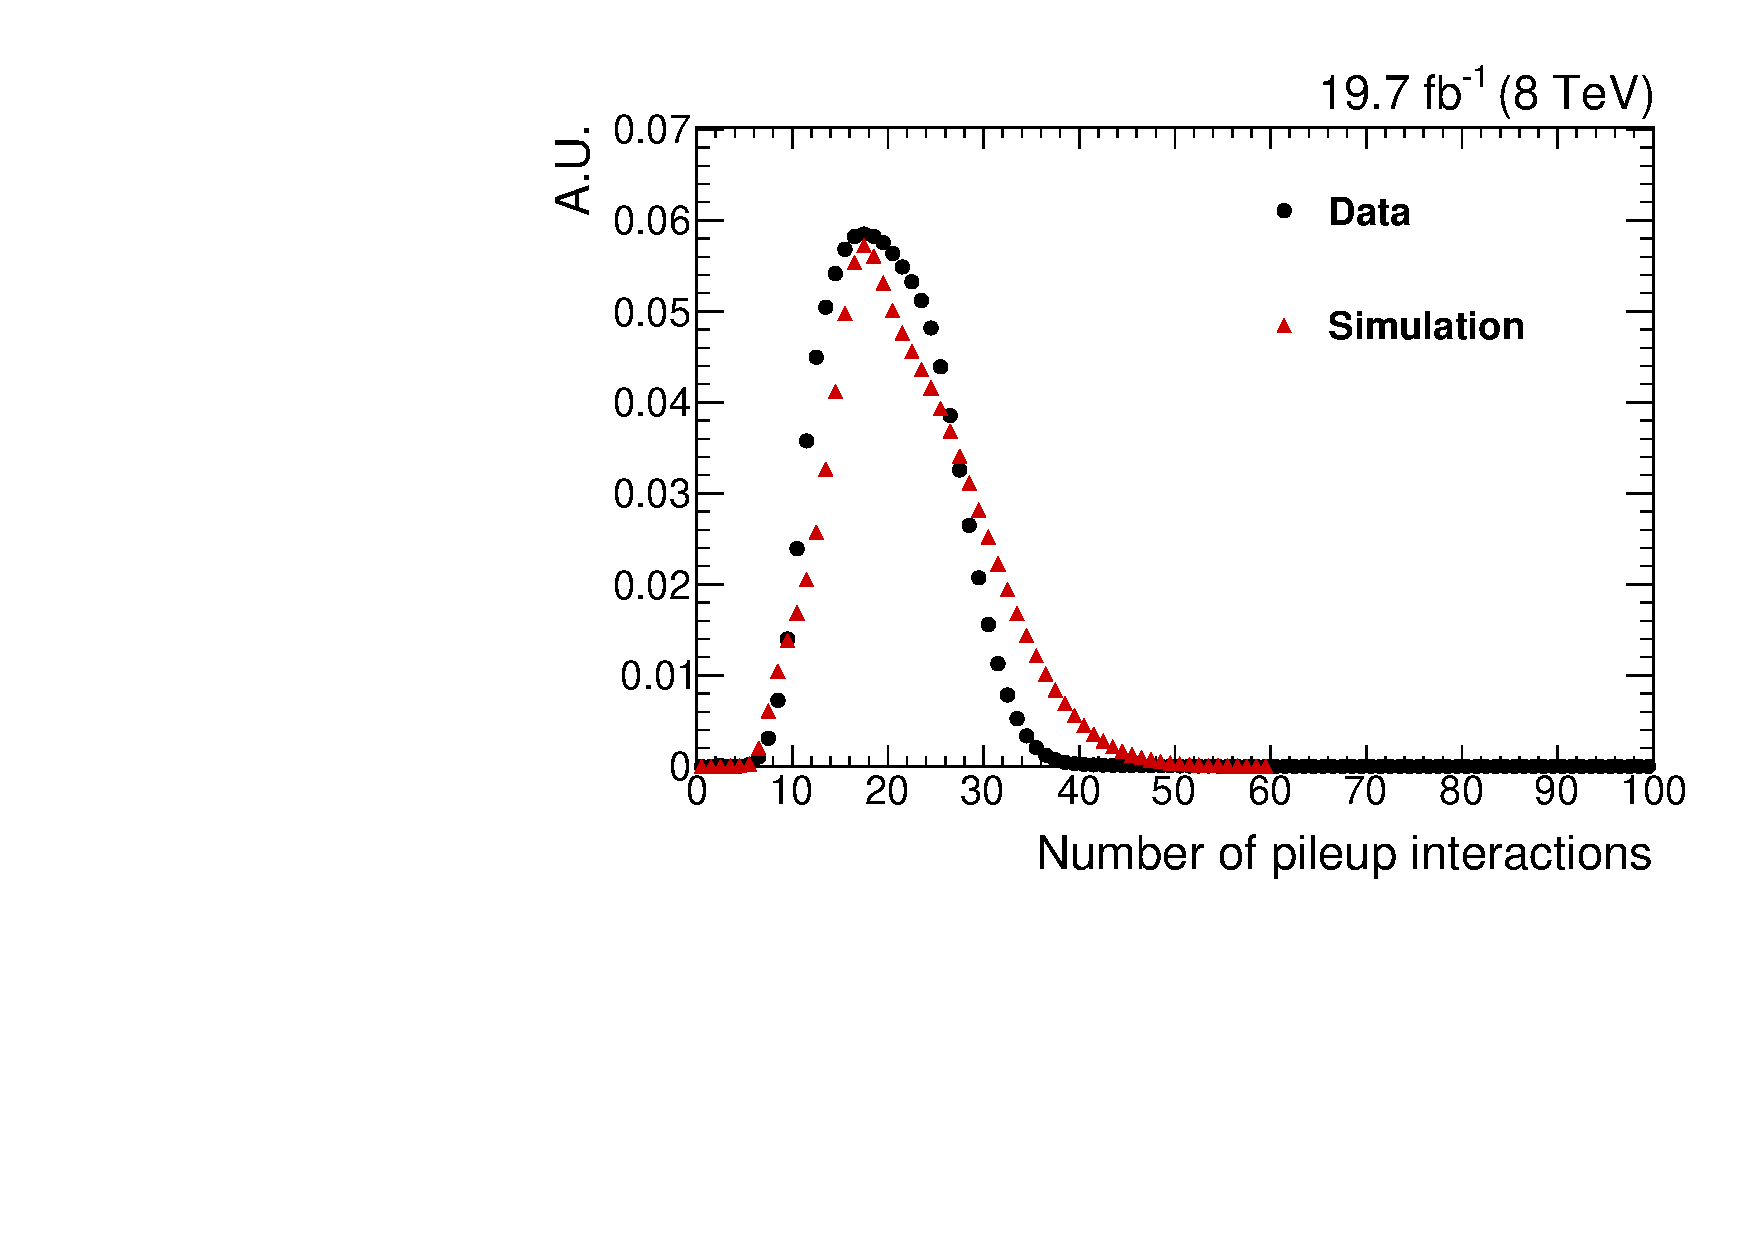
\includegraphics[width=0.48\textwidth]{figures/eventreco_reweighting/pileup_comparison}
 ~
 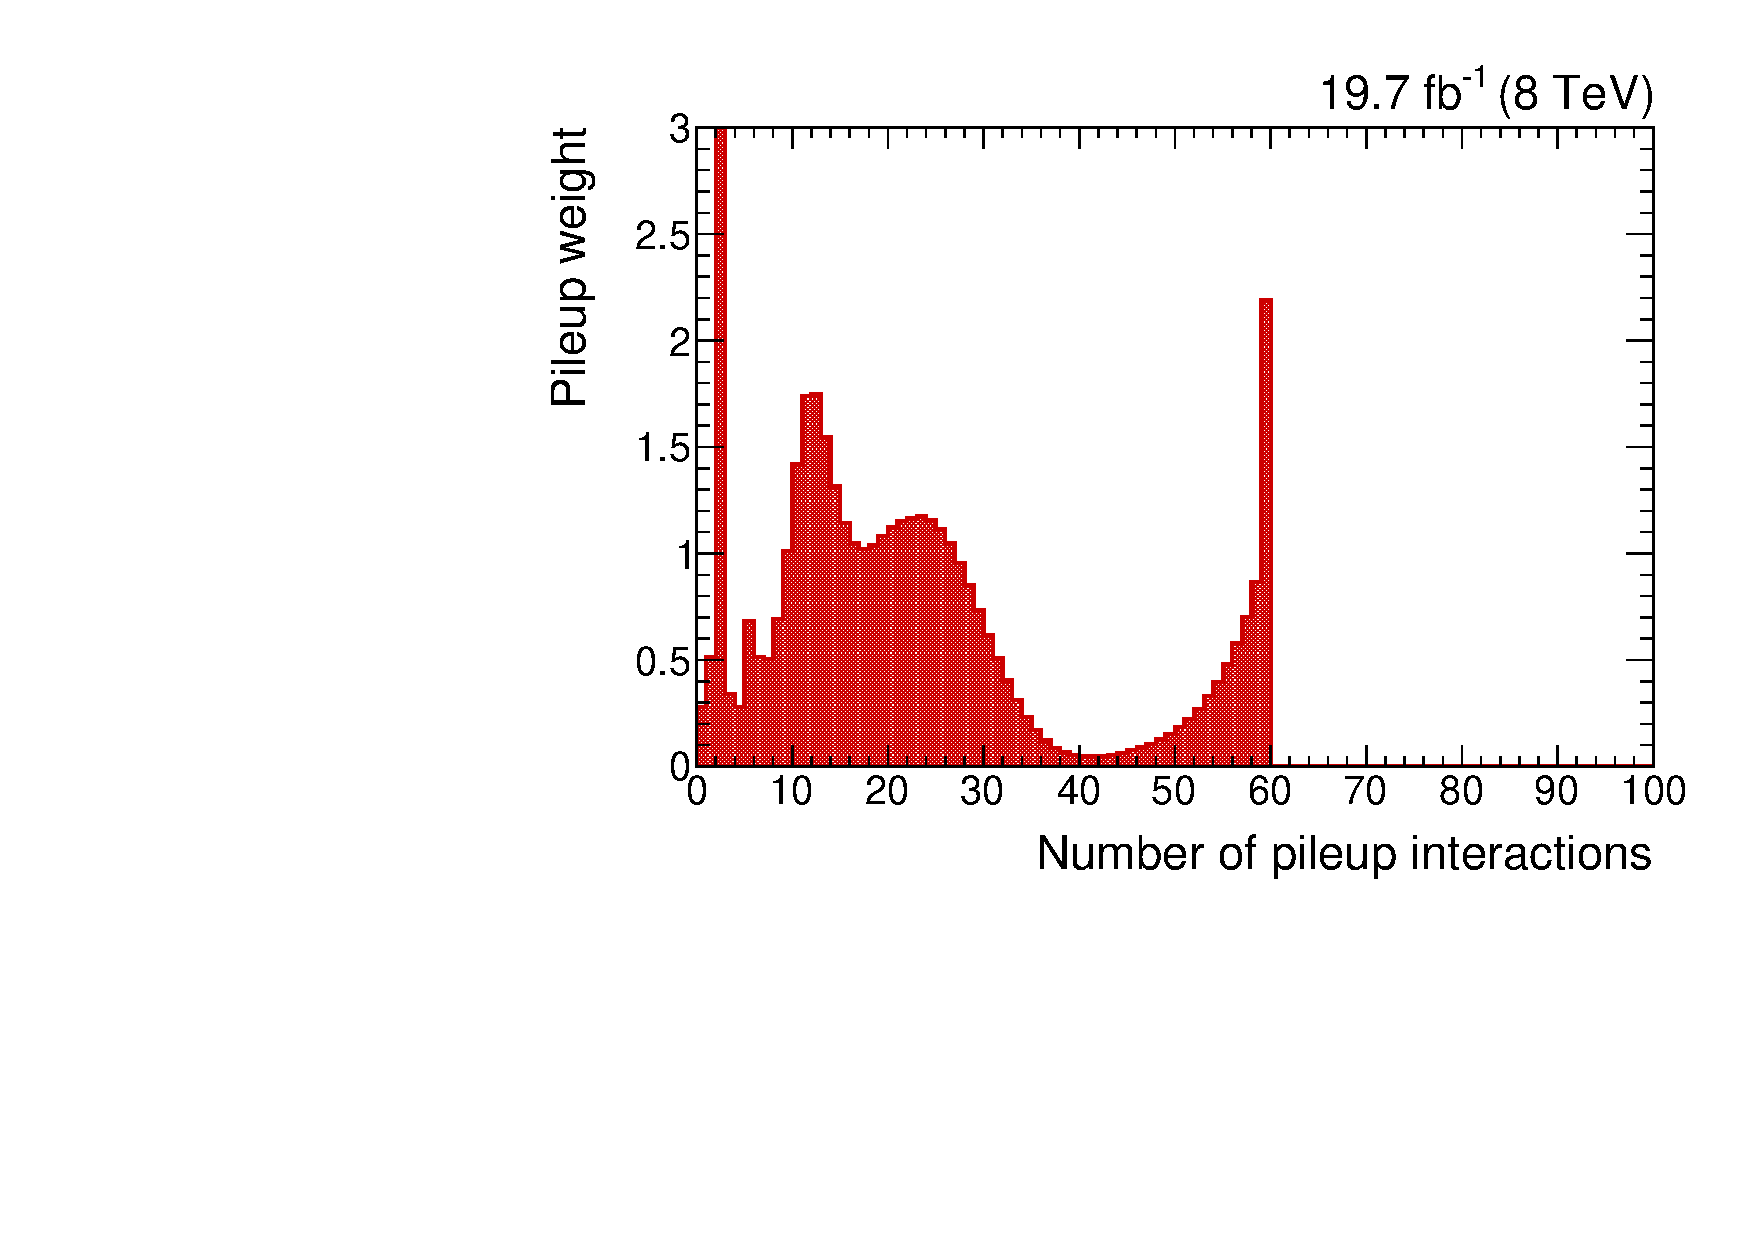
\includegraphics[width=0.48\textwidth]{figures/eventreco_reweighting/pileup_weight_comparison}
\caption{[left] Comparison of the distribution of the number of pileup interactions in data and in
simulation. 
[right] Pileup weight as a function of the number of interactions. 
\label{fig:pileup_comparison}}
\end{figure}

% TODO decide whether to add the data mc comparison for the primary vertices

% 
% As a test of the performance of the pileup reweighting, we can check the agreement between data
% and
% simulation for the distribution of the number of good primary vertices ($PV$) at different
% selection
% levels. 
% We expect to find a reasonable, although not perfect agreement as the vertex reconstruction
% efficiency depends on many things. 
% This comparison is shown in figure~\ref{fig:comparison_PV}. 
% 
% \begin{figure}
%  \includegraphics[width=0.49\textwidth]{figures/Pileup/DataMC_PV_0Lb1Ll}
%  \includegraphics[width=0.49\textwidth]{figures/Pileup/DataMC_PV_g1Mb1Ll}
% \caption{Data/MC comparison plot of the number of good primary vertices after pileup reweighting
% for
% a control region enhanced in $W+$jets (left) and enhanced in $t\bar{t}+$jets (right).
% \label{fig:comparison_PV}}
% \end{figure}
% 


\subsubsection{ISR reweighting \label{sec:event_ISRreweighting}}

Searches for new physics often rely on an initial state boost of the produced system in order to
have experimental acceptance for the signature under consideration. This is especially important
for models featuring a compressed mass spectrum. A high-\pt ISR jet can be used to suppress
background, or the boost can raise the momentum of jets or leptons in the decay chain to a level
that is detectable.
A mismodelling of the initial state radiation, or uncertainty in the modelling, will thus
directly impact the interpretation of these searches. 

A study was performed to investigate how well the ISR is
modelled in the simulation by evaluating the agreement between data and simulation in the boost \pt
for $\cPZ+$jets and $t\bar{t}$ events~\cite{Chatrchyan:2013xna,ISRreweighting}. 
For $\cPZ+$jets events the boost \pt was measured from the leptonic decay products of the $\cPZ$
boson. For $t\bar{t}$ events the ISR radiation was measured using the hadronic recoil system, which
is computed from all jets except for the $\cPqb$-tagged jets from the $t\bar{t}$ decay. 

It was found that the initial state radiation is not well modelled at high \pt, as illustrated in
Fig.~\ref{fig:ISRreweighting}. The mismodelling
can be corrected by applying a scale factor, with associated uncertainty, which was derived from the
observed disagreement. The scale factor depends on the \pt of the system recoiling against the ISR
jets. This system could be e.g. the $t\bar{t}$ system, the $\cPZ$ boson, or the $\tilde{g}\tilde{g}$
system for a SUSY event.  The uncertainty in this scale factor is taken to be the difference
between the scale factor and unity. 
The CMS SUSY group recommends that this ISR reweighting be applied to all SUSY signal samples.
The prescription is summarized in Table~\ref{tab:ISRreweighting}. 

\begin{figure}[tpb]
  \centering
  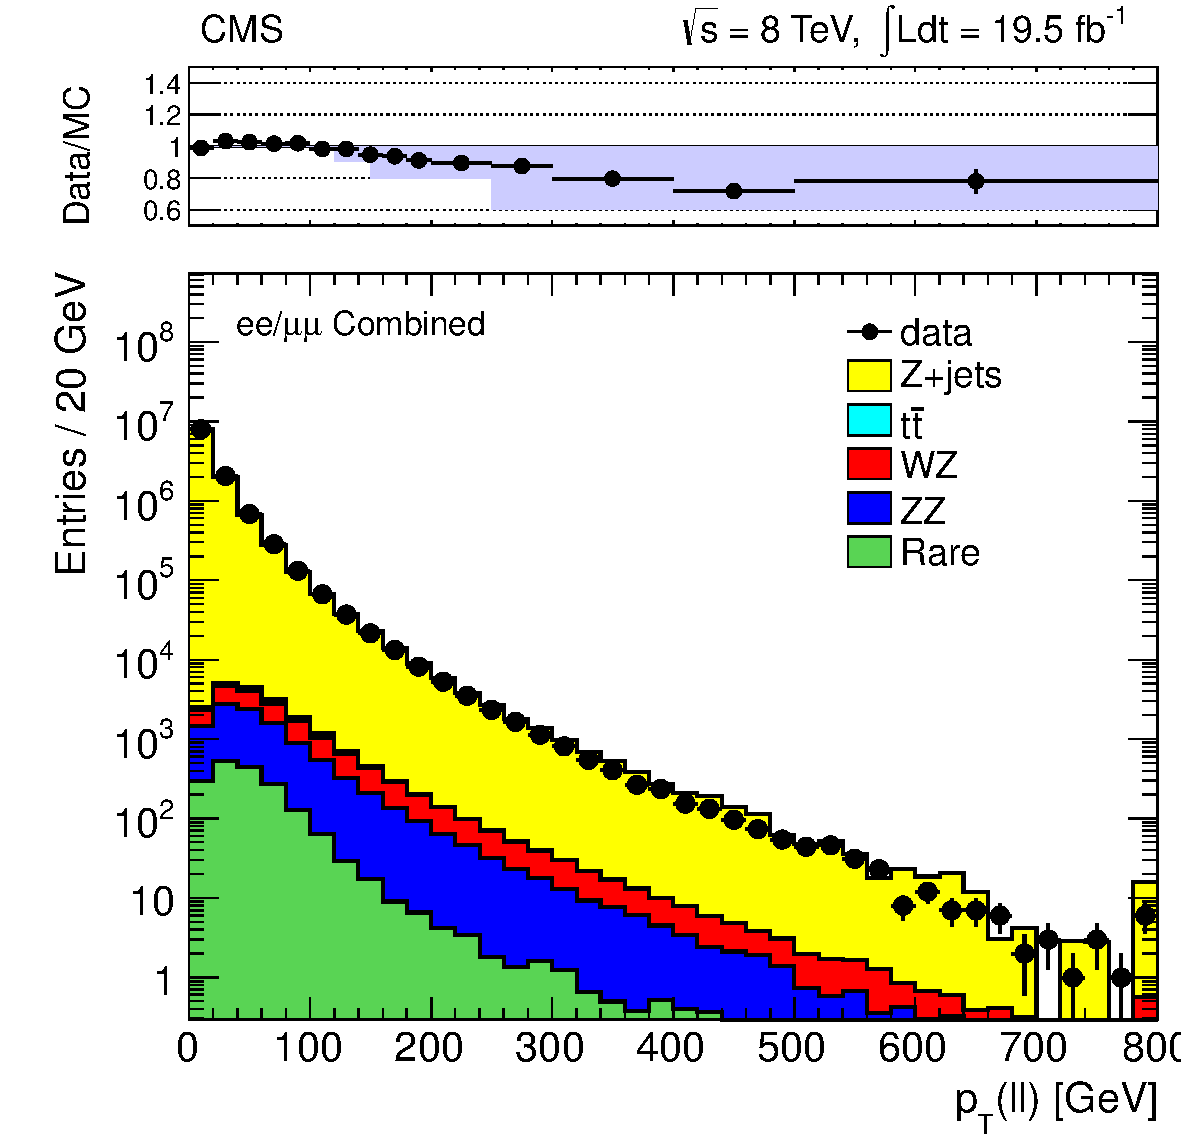
\includegraphics[width=0.7\textwidth]{figures/eventreco_reweighting/ISR_reweighting}
  \caption{ Comparison of data to simulation for the \pt of the dilepton ($ee$ or
$\mu\mu$) system in $\cPZ$+jets events. The prediction from simulation is normalized to the total
data yield to compare the shapes of the distributions. The ratio of data/simulation is shown at the
top of the figure, and the light blue band shows the weights derived for simulation and the
variation to assess systematic uncertainties. Figure from Ref.~\cite{Chatrchyan:2013xna}.
  \label{fig:ISRreweighting}}
\end{figure}

\begin{table}[htpb]
\caption{ISR reweighting prescription. \label{tab:ISRreweighting}}
\begin{center}
\begin{tabular}{c c}
\toprule
\pt of recoiling & Scale factor \\ 
system (\GeV) & \\
\midrule
$\leq 120$ & $1.00 \pm 0.00$ \\
$120 - 150 $ & $0.95 \pm 0.05$ \\
$150-250$ & $0.90 \pm 0.10$ \\
$> 250$ & $0.80 \pm 0.20$ \\
\bottomrule
\end{tabular}
\end{center}
\end{table}




\subsubsection{Top quark \texorpdfstring{$\pt$}{pt} reweighting \label{sec:event_toppt_reweighting}}

Differential top-quark-pair cross section analyses have shown that the shape of the \pt spectrum of 
top quarks in data is softer than predicted by simulation~\cite{toppt,toppt_twiki}. 
To remedy this, events are reweighted based on the \pt of the generator level $t$ and $\bar{t}$
quarks in the $t\bar{t}$ simulation.
The event weight, $w_{\rm TopPt}$, is computed as a function of the generated \pt of both the top
and anti-top quark in the event: 
\begin{equation}
w_{\rm TopPt} = \sqrt{ SF_t \cdot SF_{\bar{t}} }
\end{equation}
\begin{equation}
SF(\pt^{gen}) = \exp(a + b\, \pt^{gen})
\end{equation}
with $a = 0.156$ and $b = -0.00137$.
The uncertainty associated with this reweighting is taken to be equal to the full size of the
reweighting, which gives for the one standard deviation up and down variations of the event
weight:
\begin{align}
 +1~\sigma &: w_{\rm up} = w_{\textrm{TopPt}} \cdot w_{\textrm{TopPt}}, \\
 -1~\sigma &: w_{\rm down} = 1 .
\end{align}
The effect of this reweighting on the data/simulation agreement in a $t\bar{t}$ enriched region is
shown in Fig.~\ref{fig:TopPt}. The $x$-axis on these plots shows the razor variable $\mr$, which
will be defined in Section~\ref{sec:boost_razor}. It is clear that including this reweighting
improves the agreement. 

 
\begin{figure}[htpb]
\centering
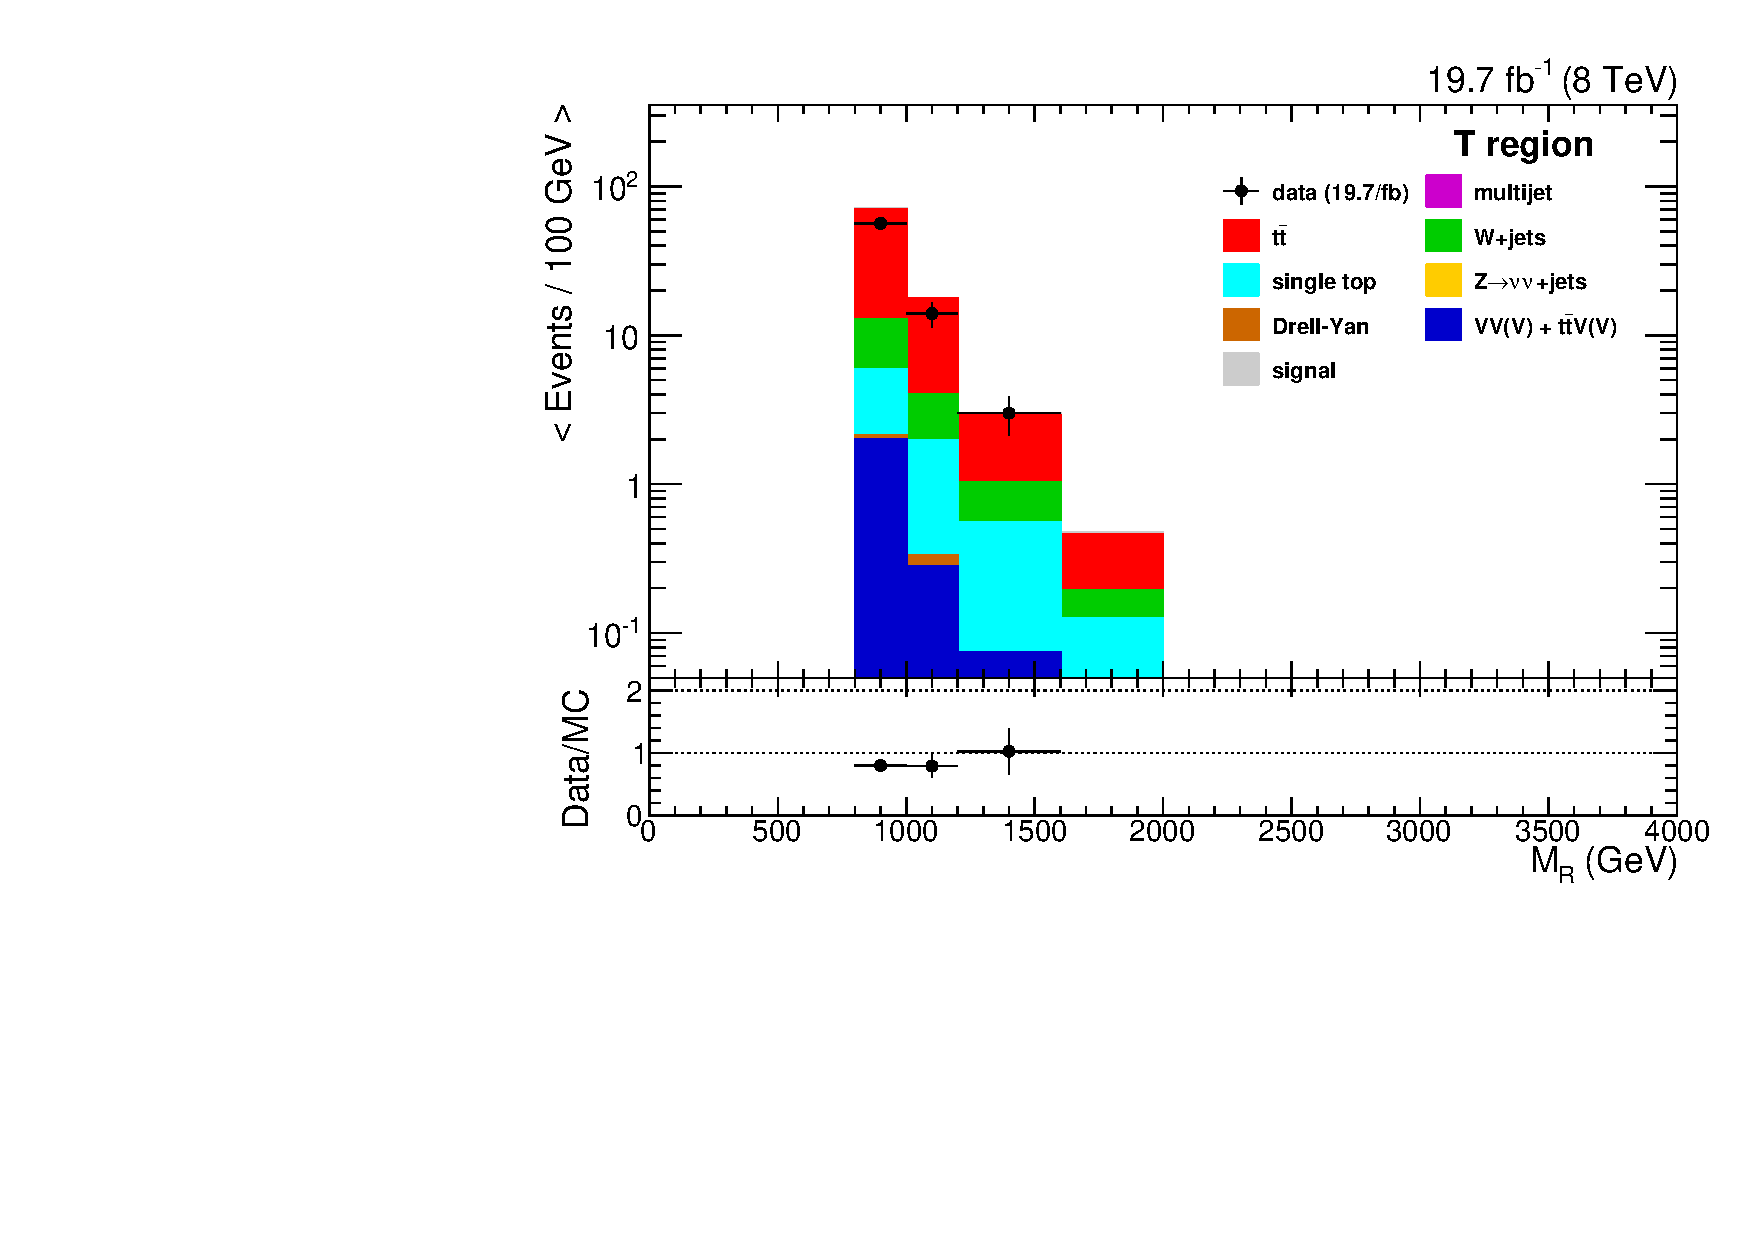
\includegraphics[width=0.48\textwidth]
{figures/razor_selection/plots_noTopPt/DataMC_MR_g1Mbg1W1LlmT100_mdPhig0p5_width}
~
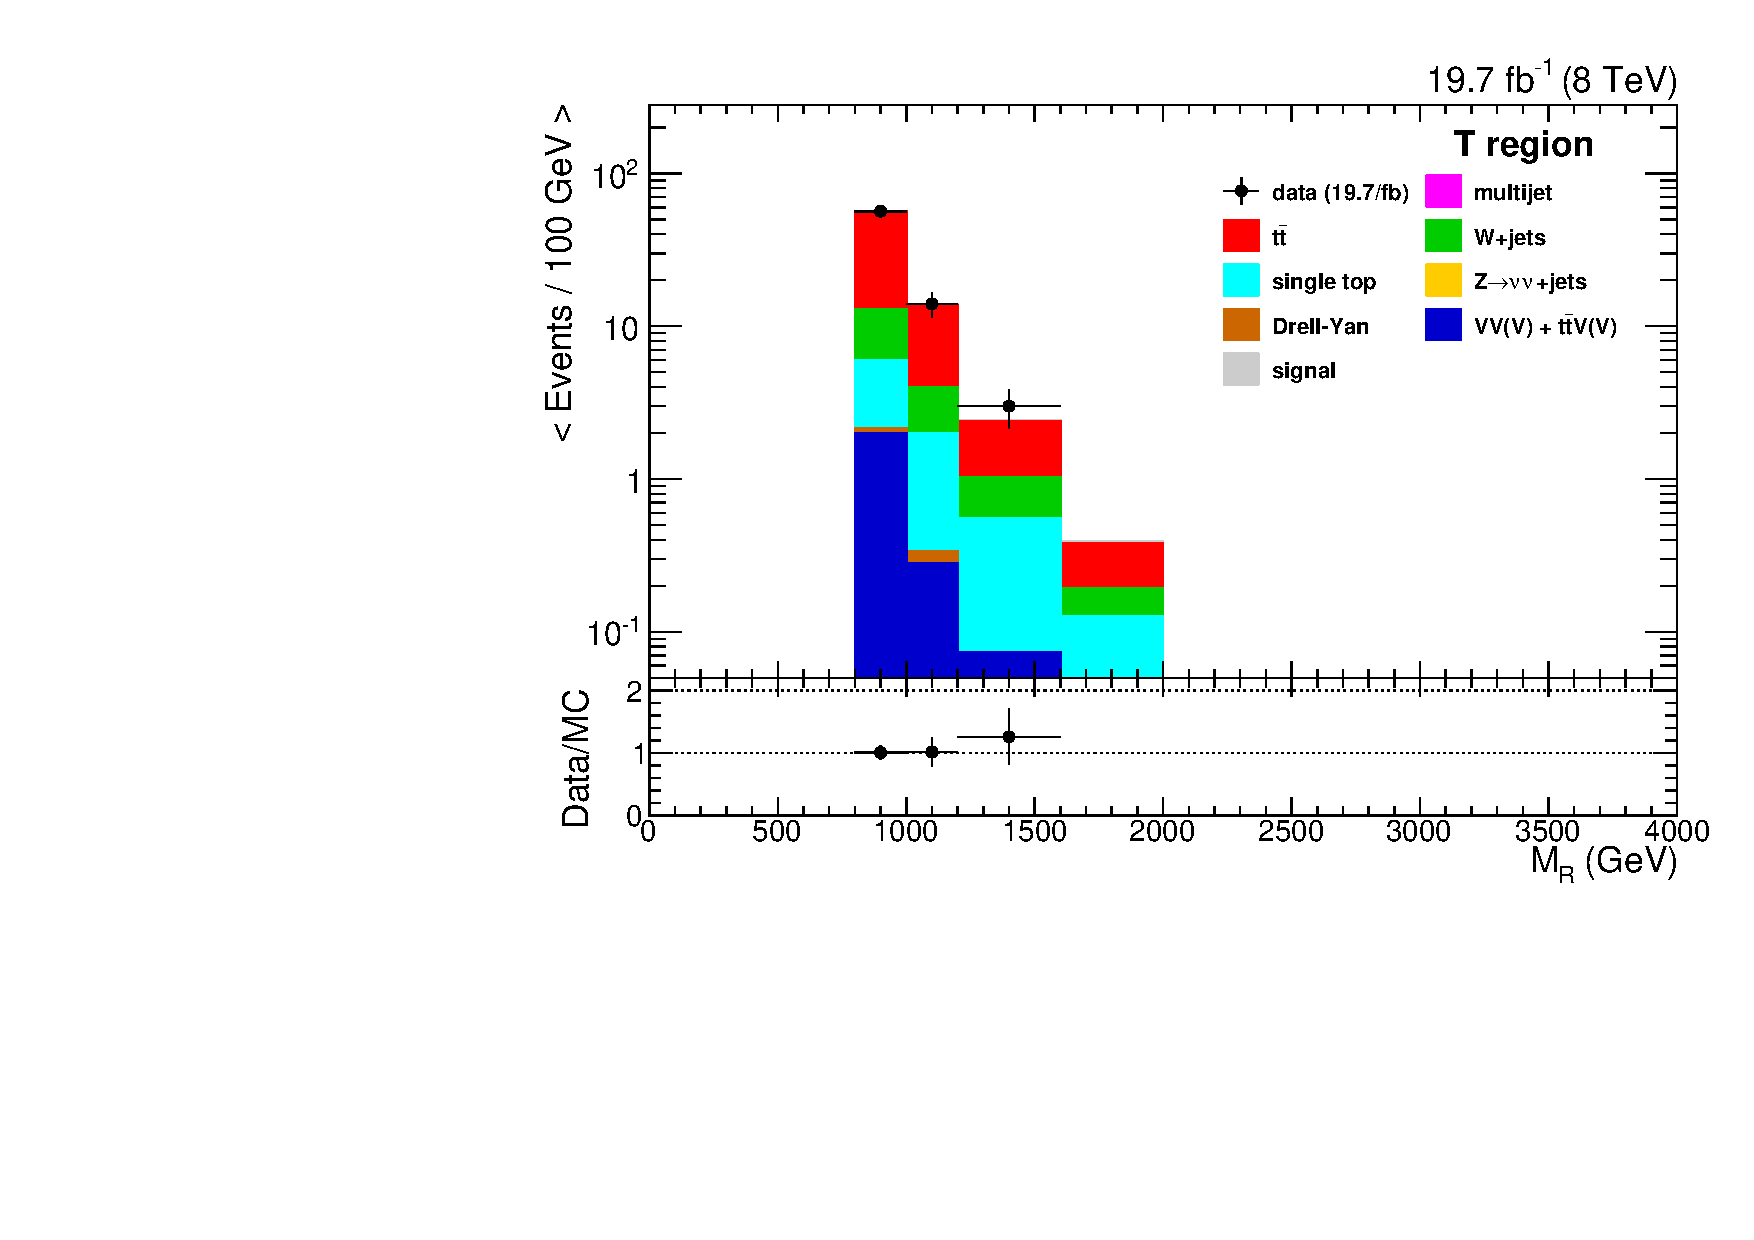
\includegraphics[width=0.48\textwidth]
{figures/razor_selection/plots/DataMC_MR_g1Mbg1W1LlmT100_mdPhig0p5_width}
\caption{Distribution of the razor variable $\mr$ in data and simulation before applying the top
\pt reweighting (left), and after (right). 
\label{fig:TopPt}}
\end{figure}




